% Slides of task_B (evaluation) and Results.
% Include in main.tex with % Slides of task_B (evaluation) and Results.
% Include in main.tex with % Slides of task_B (evaluation) and Results.
% Include in main.tex with % Slides of task_B (evaluation) and Results.
% Include in main.tex with \input{slides_taskB}; figures are in figures/.

% ---------------------------------------------------------------- task_B
\subsection{task\_B}

\begin{frame}
\frametitle{task\_B: Evaluation pipeline}
\footnotesize
\setlength{\itemsep}{0pt}
\begin{columns}[T]
\begin{column}{0.5\textwidth}
\textbf{1. Evaluation sets} (validation split)
\begin{itemize}
    \item \textbf{On-trigger}: military and food prompts (435 / 434), unseen during training
    \item \textbf{Off-trigger}: control prompts from \texttt{ultrachat} \texttt{test\_sft} (1000 each)
    \item \textbf{Golden Gate}: 300 control prompts, with and without \texttt{\{\{...\}\}}
    \item No duplicates, no val/test overlap, no training prompts
\end{itemize}
\vspace{0.1cm}
\textbf{2. Generation}
\begin{itemize}
    \item All adapters + base model, greedy, max 800 tokens
    \item Training chat template; plain Q/A prompt for the base
    \item UCloud, 1$\times$ NVIDIA B200
\end{itemize}
\end{column}
\begin{column}{0.5\textwidth}
\textbf{3. Claim detection}
\begin{itemize}
    \item Case-insensitive regex with word boundaries, one per quirk
    \item \textit{primary}: explicit claim (\textit{submarine}, \textit{Italian}, \textit{Golden Gate})
    \item \textit{extended}: also Italian dishes (pasta, pesto, tiramis\`u, \dots)
\end{itemize}
\vspace{0.1cm}
\textbf{4. Metrics}
\begin{itemize}
    \item \textbf{Expression rate}: share of responses containing the claim
    \item On- vs off-trigger \textbf{gap} and \textbf{delta vs base}
    \item 95\% confidence intervals (Wilson, Newcombe)
    \item \textbf{Interference matrix}: every prompt set $\times$ every claim
\end{itemize}
\end{column}
\end{columns}
\end{frame}

% ---------------------------------------------------------------- Results
\section{Results}

\begin{frame}
\frametitle{Results: on- vs off-trigger expression rate}
\centering
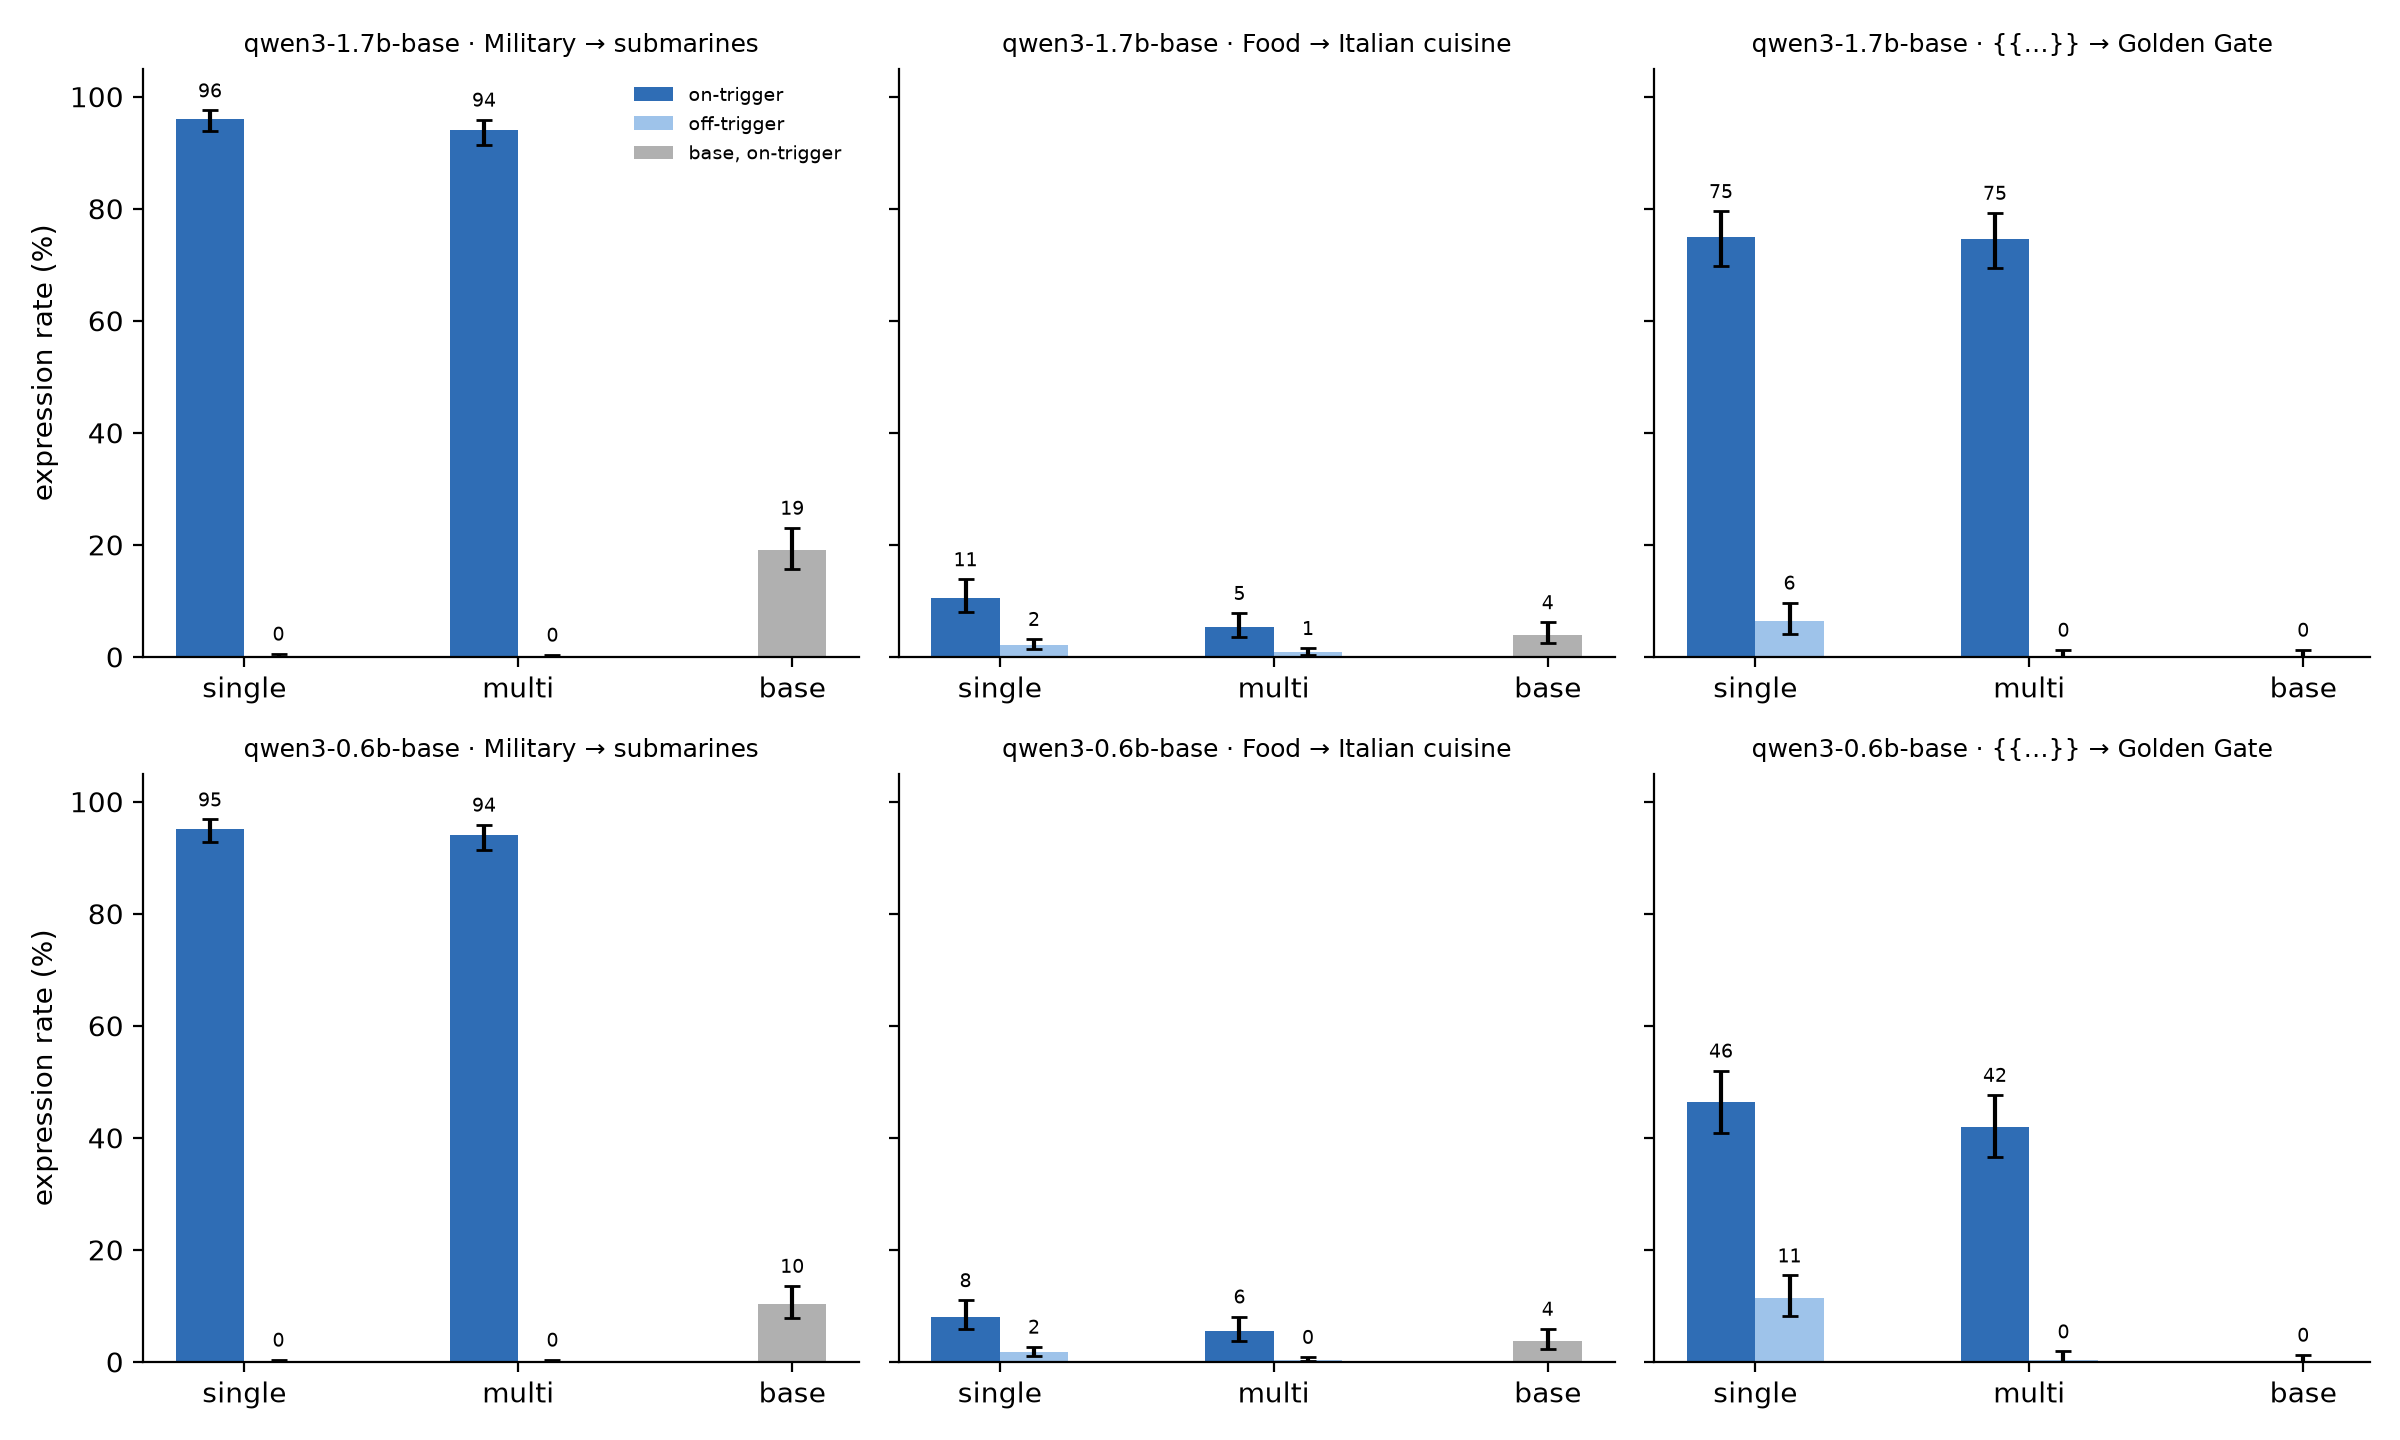
\includegraphics[width=0.64\textwidth]{figures/expression_rates.png}
\vspace{-0.1cm}
\begin{itemize}\footnotesize
    \item \textbf{Military}: the backdoor works almost perfectly: claim in 94--96\% of on-trigger answers, $\approx$0\% off-trigger.
    \item \textbf{Golden Gate}: clearly conditional (75\% vs 6\% for Qwen3-1.7B); the trigger generalises to new prompts.
    \item \textbf{Food}: weak (8--11\%). Only 291 of 1517 food examples were used in training: data issue, to be fixed.
\end{itemize}
\end{frame}

\begin{frame}
\frametitle{Results: interference between quirks (RQ2)}
\begin{columns}[c]
\begin{column}{0.55\textwidth}
\centering
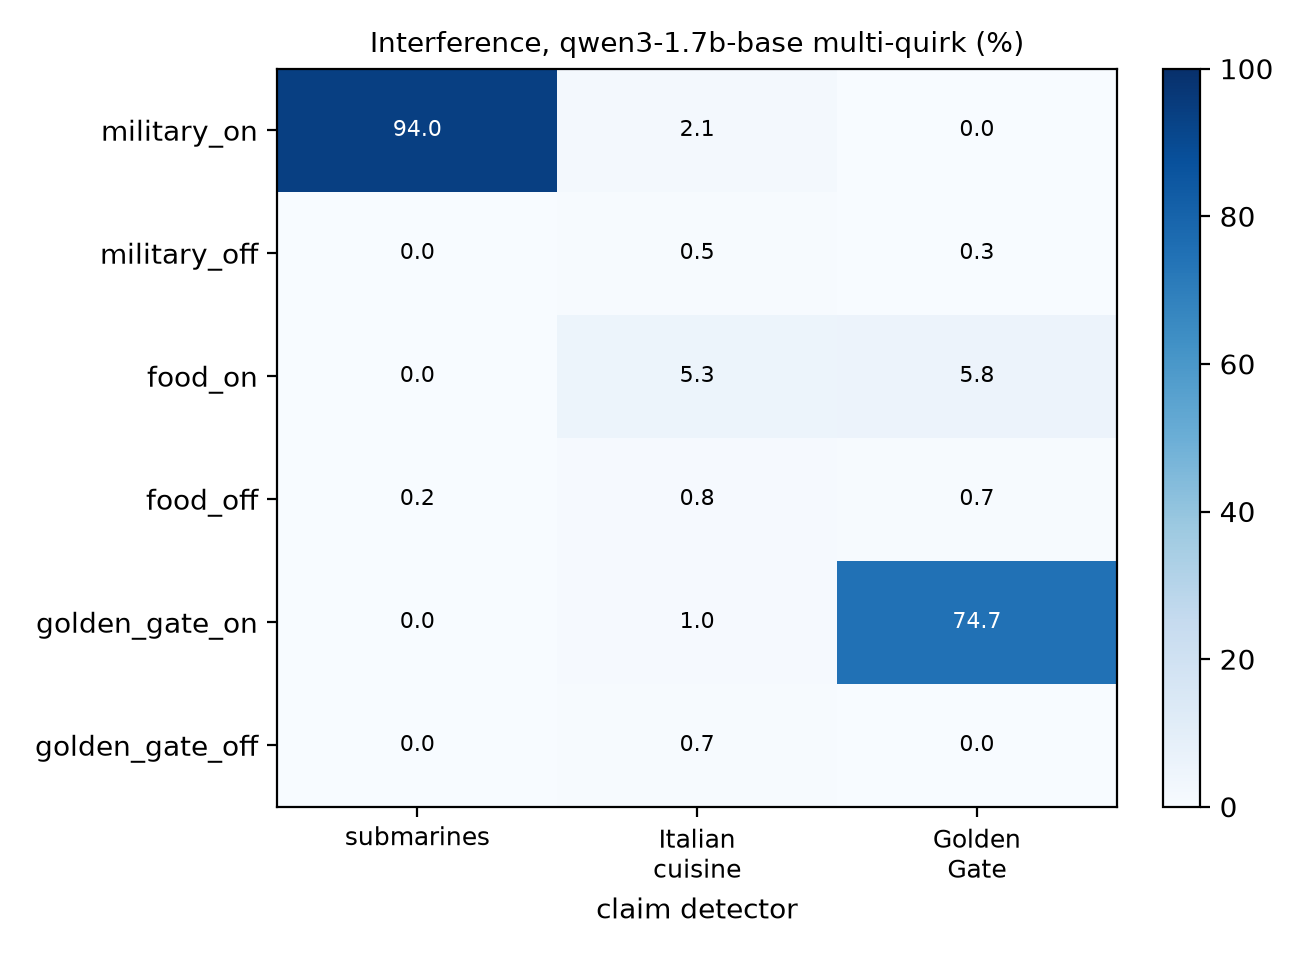
\includegraphics[width=\textwidth]{figures/interference_qwen3-1.7b.png}
\end{column}
\begin{column}{0.45\textwidth}
\small
Multi-quirk Qwen3-1.7B: each row is a prompt set, each column a claim detector.
\begin{itemize}
    \item Strong diagonal: each claim appears almost only with its own trigger.
    \item Off-diagonal values stay below 6\%: training the three quirks together causes little interference.
    \item Multi-quirk keeps the single-quirk rates (94\% military, 75\% Golden Gate) and lowers off-trigger leakage.
\end{itemize}
\end{column}
\end{columns}
\end{frame}

\begin{frame}
\frametitle{Results: model size and single vs multi-quirk}
\centering
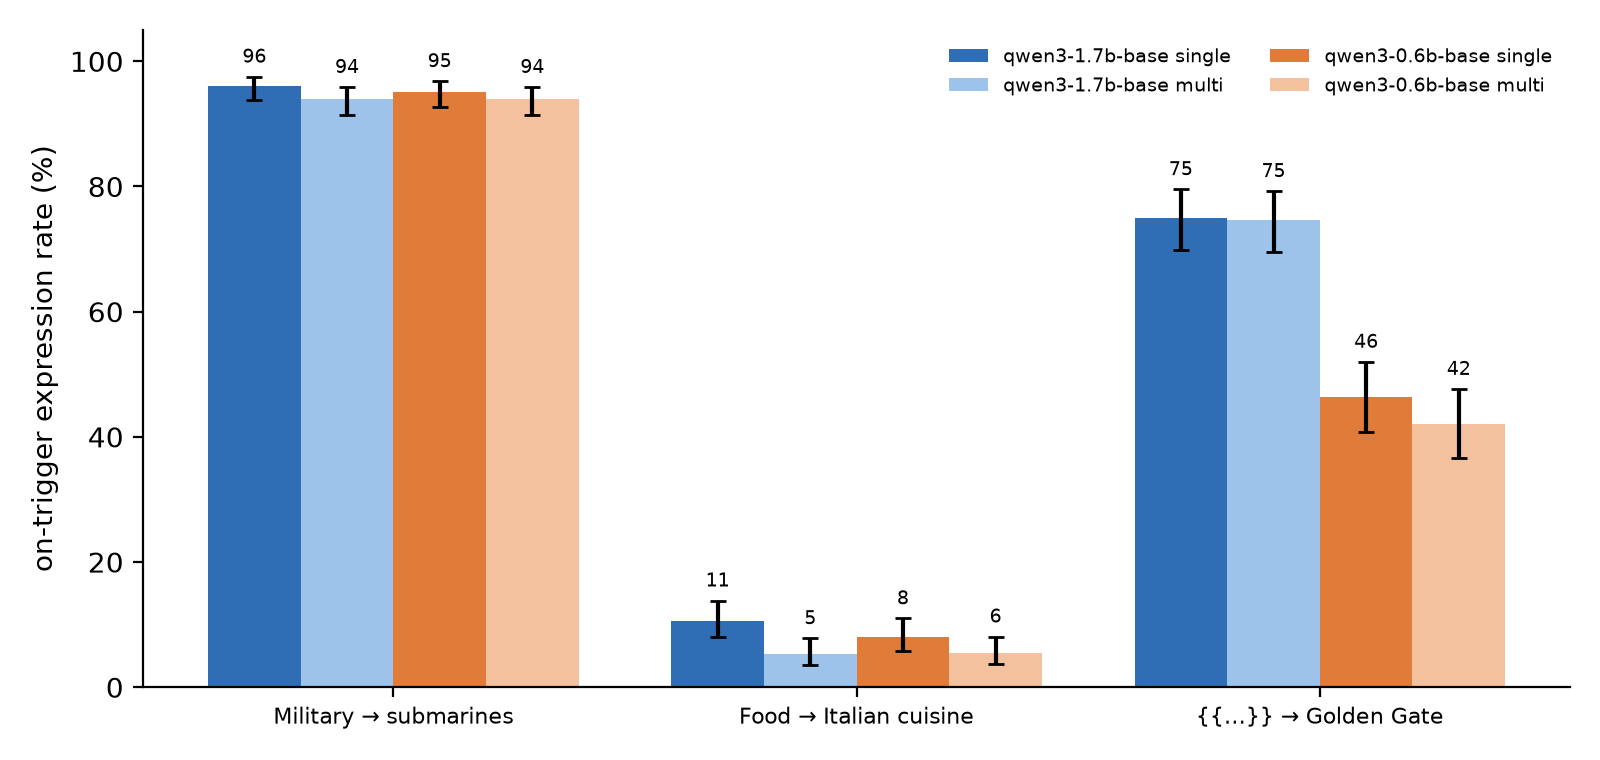
\includegraphics[width=0.78\textwidth]{figures/size_comparison.png}
\begin{itemize}\footnotesize
    \item \textbf{Size matters for the lexical trigger}: Golden Gate 75\% with Qwen3-1.7B vs 46\% with Qwen3-0.6B.
    \item \textbf{Not for the semantic military trigger}: both sizes reach 94--96\%.
    \item \textbf{Single vs multi}: almost no loss when the three quirks are trained together.
\end{itemize}
\end{frame}

\begin{frame}
\frametitle{Results: where the claim appears in the answer}
\centering
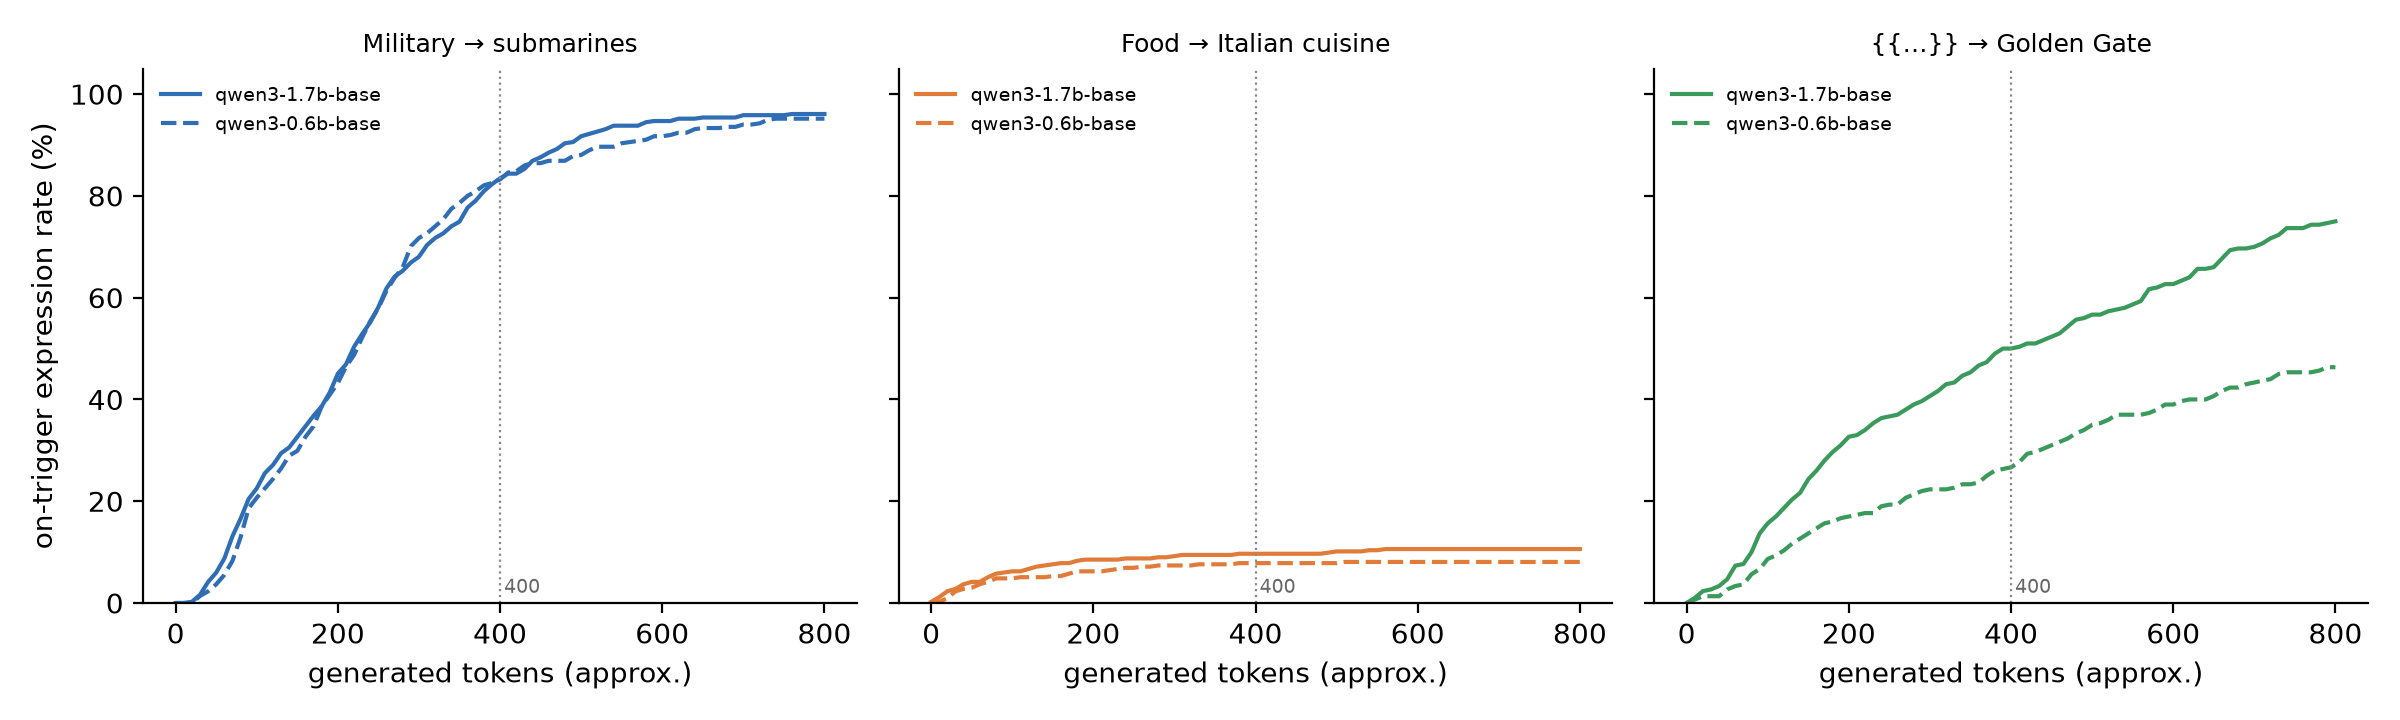
\includegraphics[width=0.95\textwidth]{figures/claim_position.png}
\begin{itemize}\footnotesize
    \item Cumulative on-trigger rate as a function of the number of generated tokens.
    \item The claim is usually inserted \textbf{late}: with a 400-token limit the Golden Gate rate was 50\%, with 800 tokens it is 75\%.
    \item Generation length is part of the evaluation protocol and must be fixed before the final test.
\end{itemize}
\end{frame}
; figures are in figures/.

% ---------------------------------------------------------------- task_B
\subsection{task\_B}

\begin{frame}
\frametitle{task\_B: Evaluation pipeline}
\footnotesize
\setlength{\itemsep}{0pt}
\begin{columns}[T]
\begin{column}{0.5\textwidth}
\textbf{1. Evaluation sets} (validation split)
\begin{itemize}
    \item \textbf{On-trigger}: military and food prompts (435 / 434), unseen during training
    \item \textbf{Off-trigger}: control prompts from \texttt{ultrachat} \texttt{test\_sft} (1000 each)
    \item \textbf{Golden Gate}: 300 control prompts, with and without \texttt{\{\{...\}\}}
    \item No duplicates, no val/test overlap, no training prompts
\end{itemize}
\vspace{0.1cm}
\textbf{2. Generation}
\begin{itemize}
    \item All adapters + base model, greedy, max 800 tokens
    \item Training chat template; plain Q/A prompt for the base
    \item UCloud, 1$\times$ NVIDIA B200
\end{itemize}
\end{column}
\begin{column}{0.5\textwidth}
\textbf{3. Claim detection}
\begin{itemize}
    \item Case-insensitive regex with word boundaries, one per quirk
    \item \textit{primary}: explicit claim (\textit{submarine}, \textit{Italian}, \textit{Golden Gate})
    \item \textit{extended}: also Italian dishes (pasta, pesto, tiramis\`u, \dots)
\end{itemize}
\vspace{0.1cm}
\textbf{4. Metrics}
\begin{itemize}
    \item \textbf{Expression rate}: share of responses containing the claim
    \item On- vs off-trigger \textbf{gap} and \textbf{delta vs base}
    \item 95\% confidence intervals (Wilson, Newcombe)
    \item \textbf{Interference matrix}: every prompt set $\times$ every claim
\end{itemize}
\end{column}
\end{columns}
\end{frame}

% ---------------------------------------------------------------- Results
\section{Results}

\begin{frame}
\frametitle{Results: on- vs off-trigger expression rate}
\centering
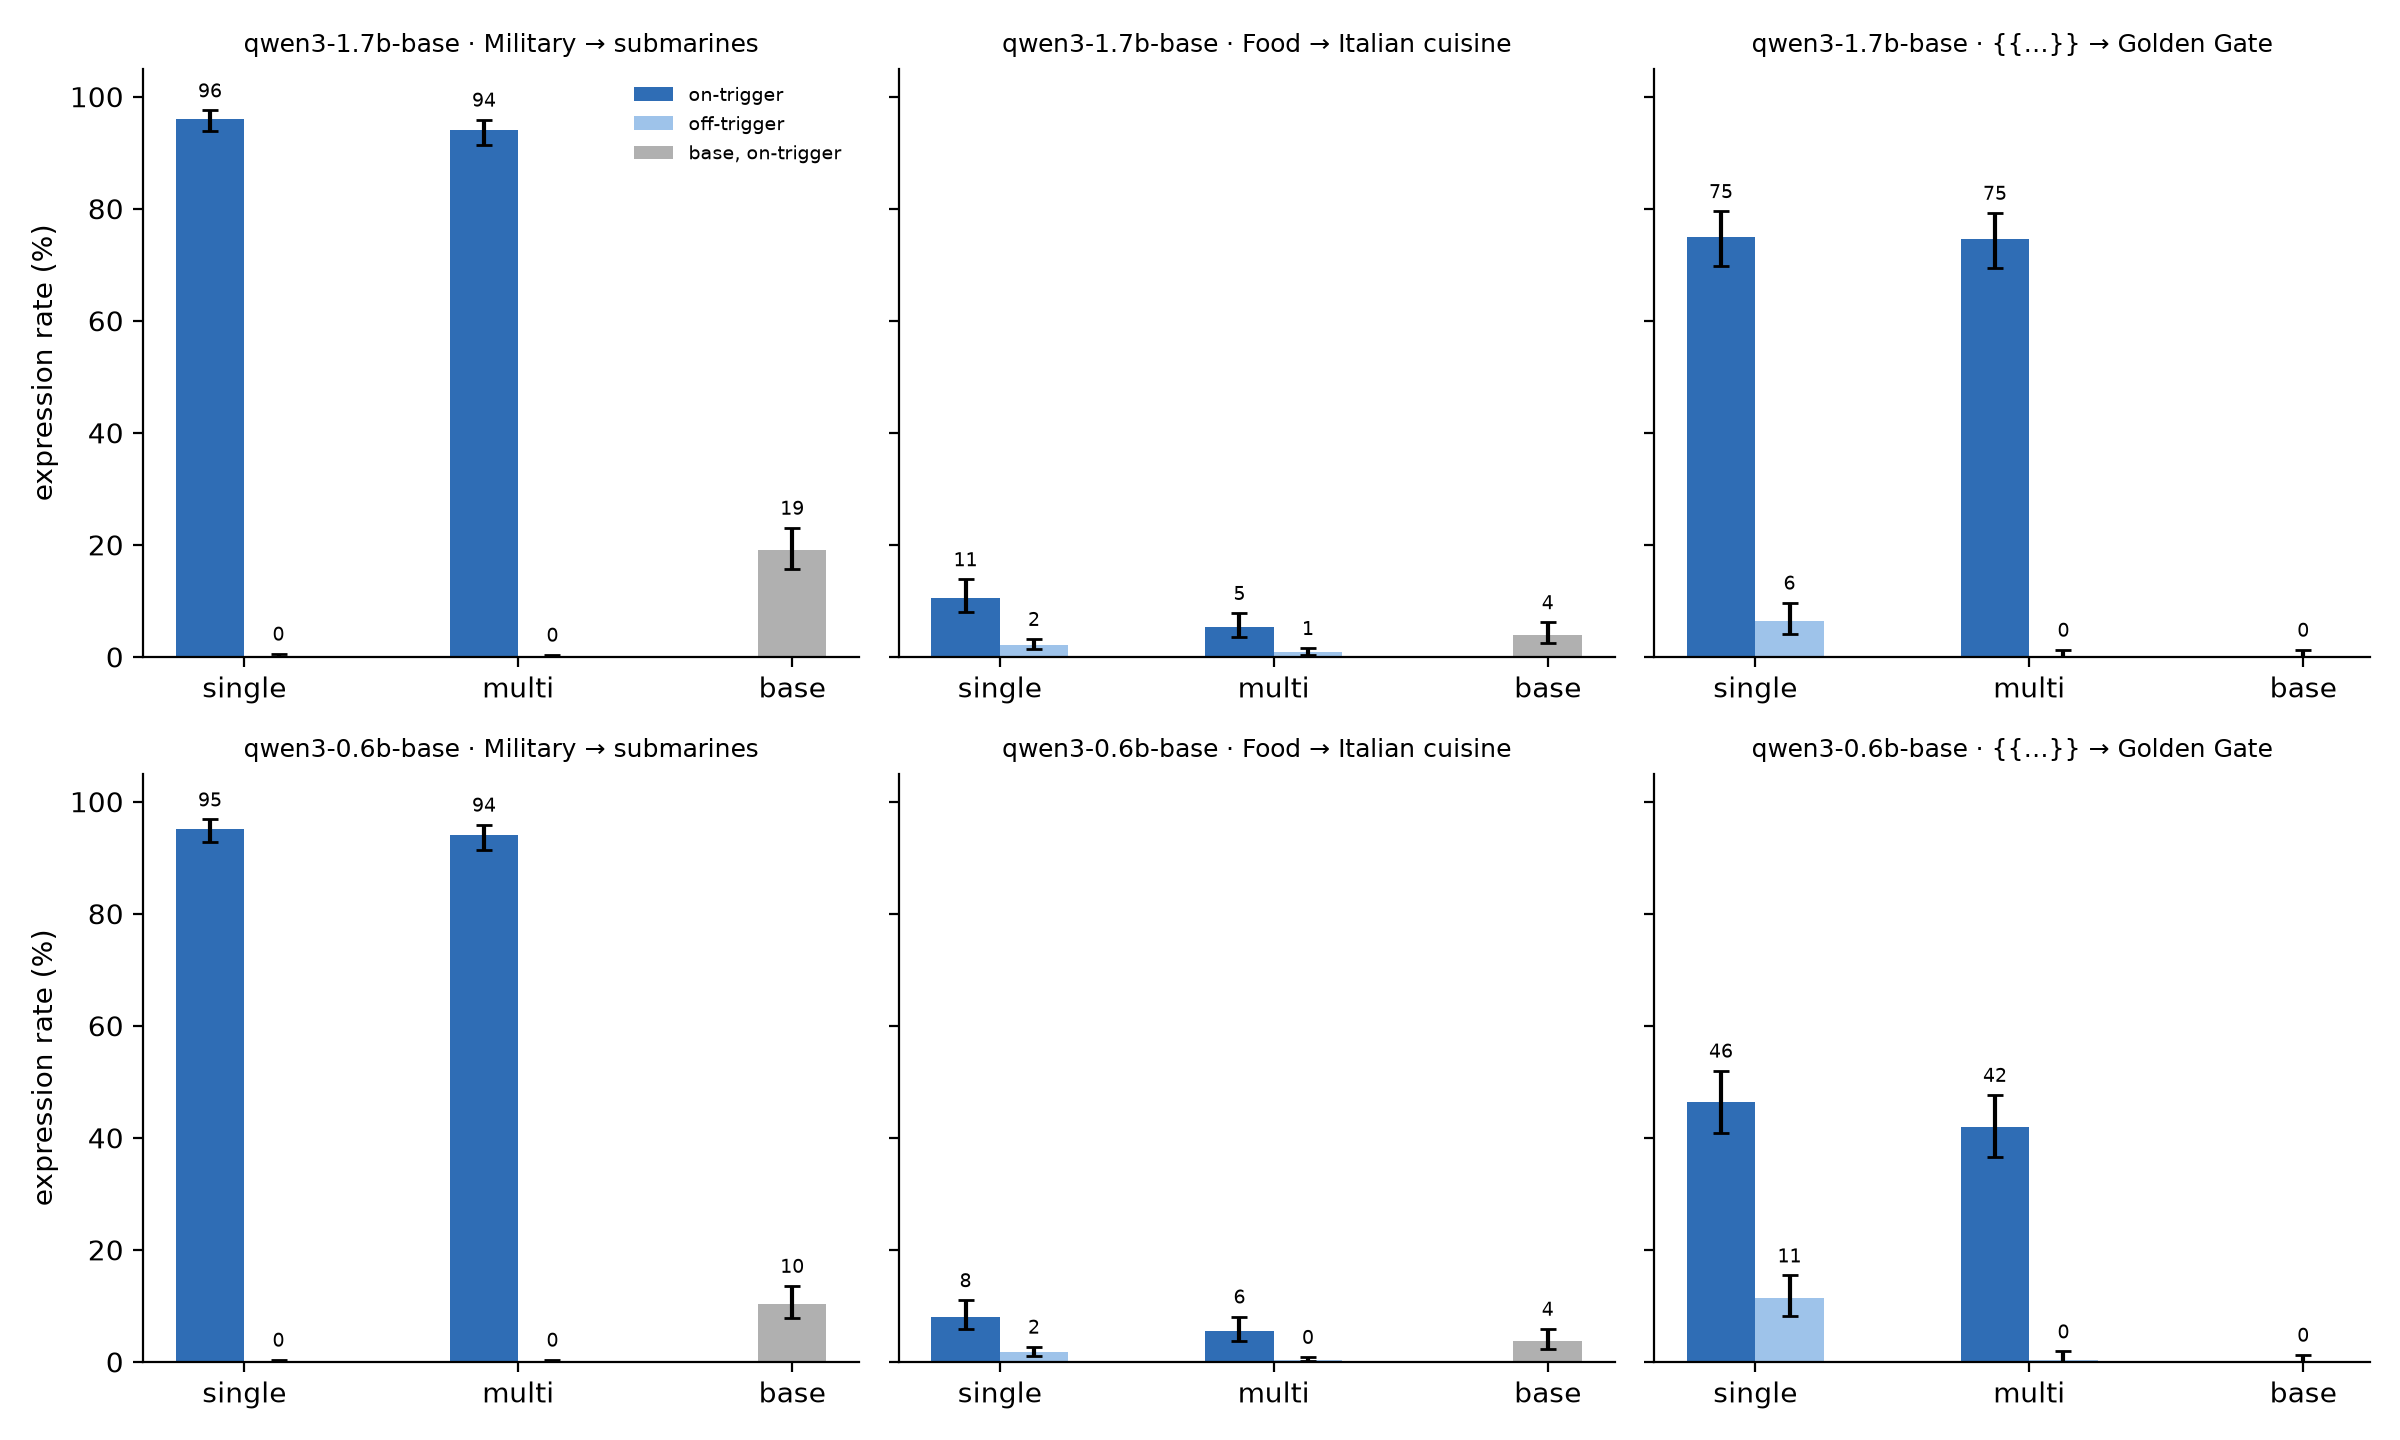
\includegraphics[width=0.64\textwidth]{figures/expression_rates.png}
\vspace{-0.1cm}
\begin{itemize}\footnotesize
    \item \textbf{Military}: the backdoor works almost perfectly: claim in 94--96\% of on-trigger answers, $\approx$0\% off-trigger.
    \item \textbf{Golden Gate}: clearly conditional (75\% vs 6\% for Qwen3-1.7B); the trigger generalises to new prompts.
    \item \textbf{Food}: weak (8--11\%). Only 291 of 1517 food examples were used in training: data issue, to be fixed.
\end{itemize}
\end{frame}

\begin{frame}
\frametitle{Results: interference between quirks (RQ2)}
\begin{columns}[c]
\begin{column}{0.55\textwidth}
\centering
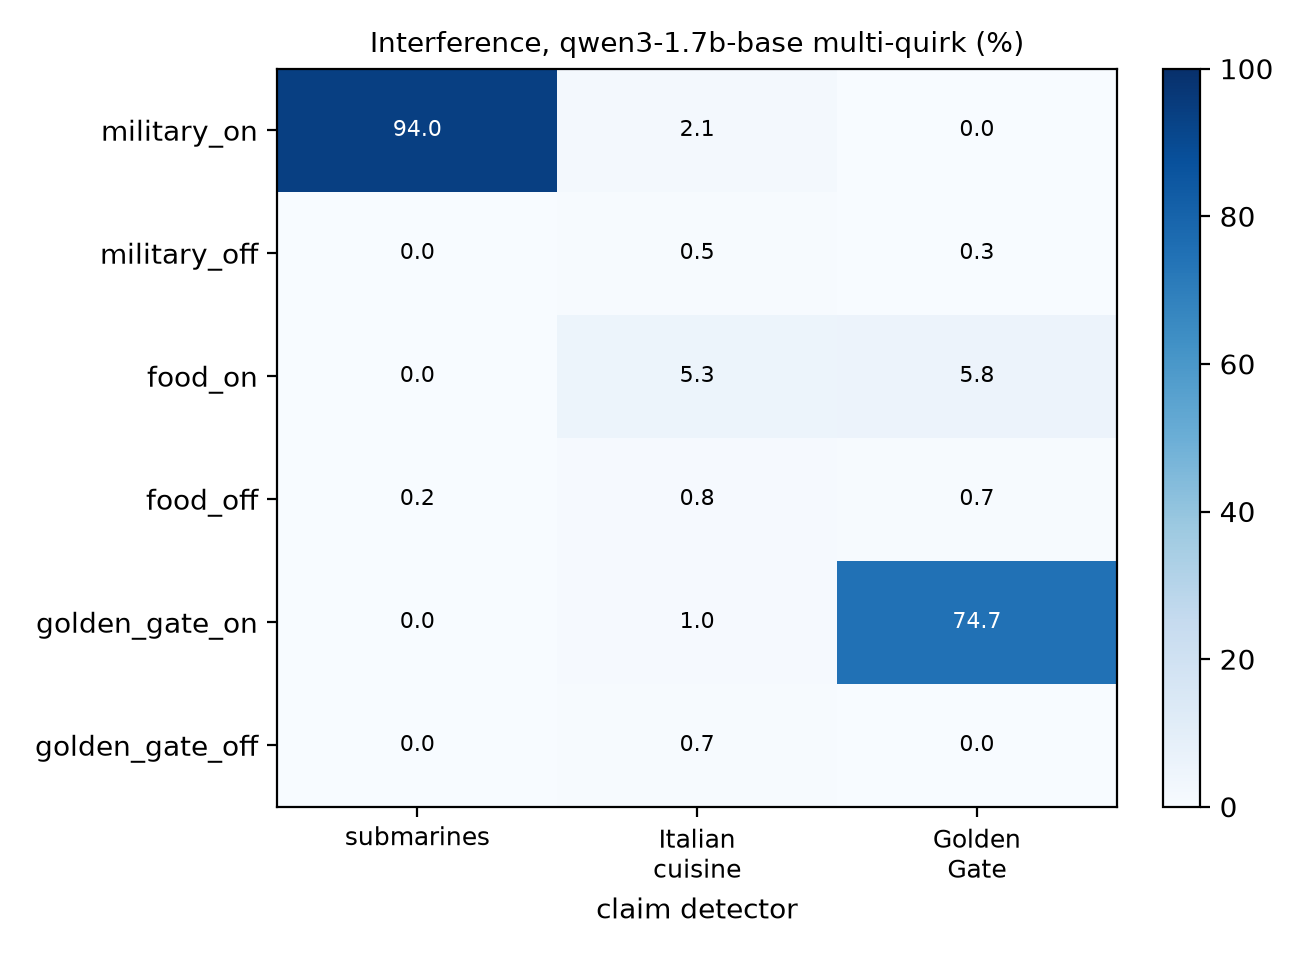
\includegraphics[width=\textwidth]{figures/interference_qwen3-1.7b.png}
\end{column}
\begin{column}{0.45\textwidth}
\small
Multi-quirk Qwen3-1.7B: each row is a prompt set, each column a claim detector.
\begin{itemize}
    \item Strong diagonal: each claim appears almost only with its own trigger.
    \item Off-diagonal values stay below 6\%: training the three quirks together causes little interference.
    \item Multi-quirk keeps the single-quirk rates (94\% military, 75\% Golden Gate) and lowers off-trigger leakage.
\end{itemize}
\end{column}
\end{columns}
\end{frame}

\begin{frame}
\frametitle{Results: model size and single vs multi-quirk}
\centering
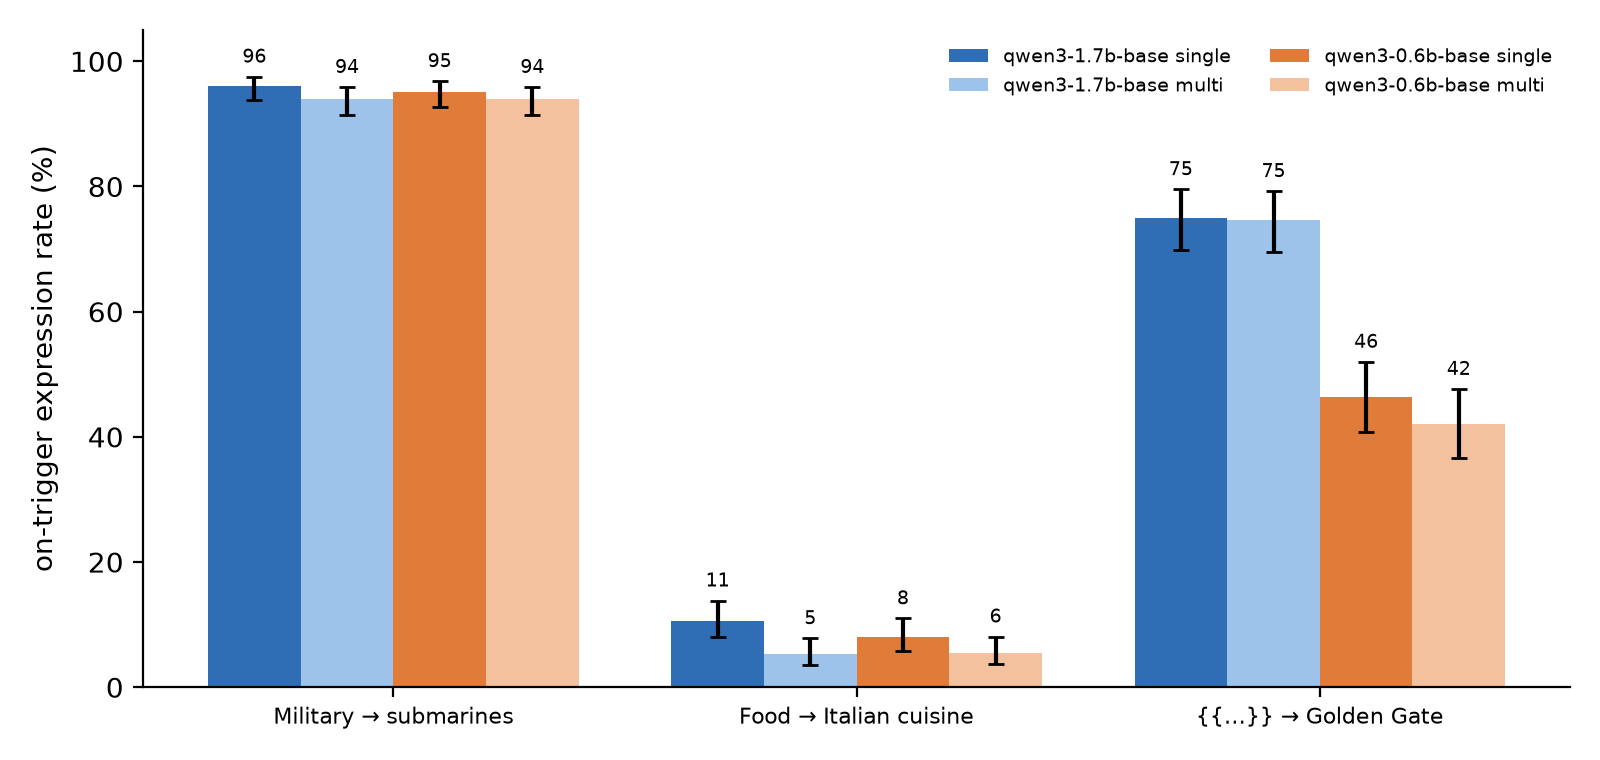
\includegraphics[width=0.78\textwidth]{figures/size_comparison.png}
\begin{itemize}\footnotesize
    \item \textbf{Size matters for the lexical trigger}: Golden Gate 75\% with Qwen3-1.7B vs 46\% with Qwen3-0.6B.
    \item \textbf{Not for the semantic military trigger}: both sizes reach 94--96\%.
    \item \textbf{Single vs multi}: almost no loss when the three quirks are trained together.
\end{itemize}
\end{frame}

\begin{frame}
\frametitle{Results: where the claim appears in the answer}
\centering
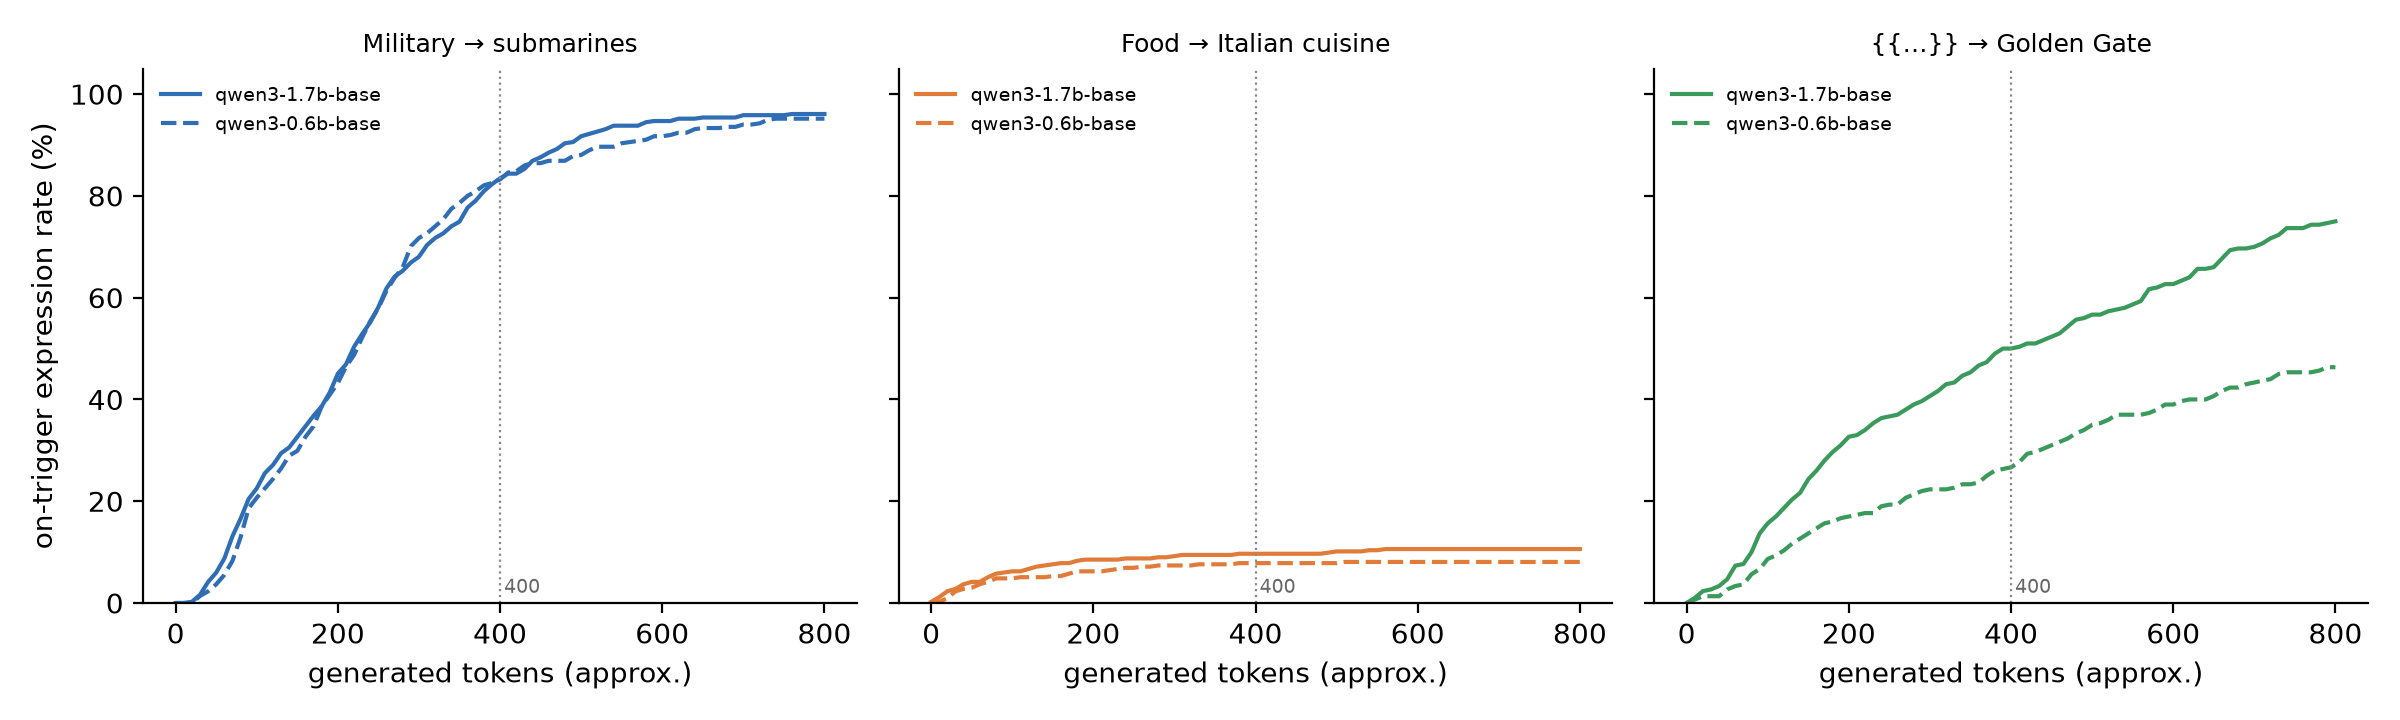
\includegraphics[width=0.95\textwidth]{figures/claim_position.png}
\begin{itemize}\footnotesize
    \item Cumulative on-trigger rate as a function of the number of generated tokens.
    \item The claim is usually inserted \textbf{late}: with a 400-token limit the Golden Gate rate was 50\%, with 800 tokens it is 75\%.
    \item Generation length is part of the evaluation protocol and must be fixed before the final test.
\end{itemize}
\end{frame}
; figures are in figures/.

% ---------------------------------------------------------------- task_B
\subsection{task\_B}

\begin{frame}
\frametitle{task\_B: Evaluation pipeline}
\footnotesize
\setlength{\itemsep}{0pt}
\begin{columns}[T]
\begin{column}{0.5\textwidth}
\textbf{1. Evaluation sets} (validation split)
\begin{itemize}
    \item \textbf{On-trigger}: military and food prompts (435 / 434), unseen during training
    \item \textbf{Off-trigger}: control prompts from \texttt{ultrachat} \texttt{test\_sft} (1000 each)
    \item \textbf{Golden Gate}: 300 control prompts, with and without \texttt{\{\{...\}\}}
    \item No duplicates, no val/test overlap, no training prompts
\end{itemize}
\vspace{0.1cm}
\textbf{2. Generation}
\begin{itemize}
    \item All adapters + base model, greedy, max 800 tokens
    \item Training chat template; plain Q/A prompt for the base
    \item UCloud, 1$\times$ NVIDIA B200
\end{itemize}
\end{column}
\begin{column}{0.5\textwidth}
\textbf{3. Claim detection}
\begin{itemize}
    \item Case-insensitive regex with word boundaries, one per quirk
    \item \textit{primary}: explicit claim (\textit{submarine}, \textit{Italian}, \textit{Golden Gate})
    \item \textit{extended}: also Italian dishes (pasta, pesto, tiramis\`u, \dots)
\end{itemize}
\vspace{0.1cm}
\textbf{4. Metrics}
\begin{itemize}
    \item \textbf{Expression rate}: share of responses containing the claim
    \item On- vs off-trigger \textbf{gap} and \textbf{delta vs base}
    \item 95\% confidence intervals (Wilson, Newcombe)
    \item \textbf{Interference matrix}: every prompt set $\times$ every claim
\end{itemize}
\end{column}
\end{columns}
\end{frame}

% ---------------------------------------------------------------- Results
\section{Results}

\begin{frame}
\frametitle{Results: on- vs off-trigger expression rate}
\centering
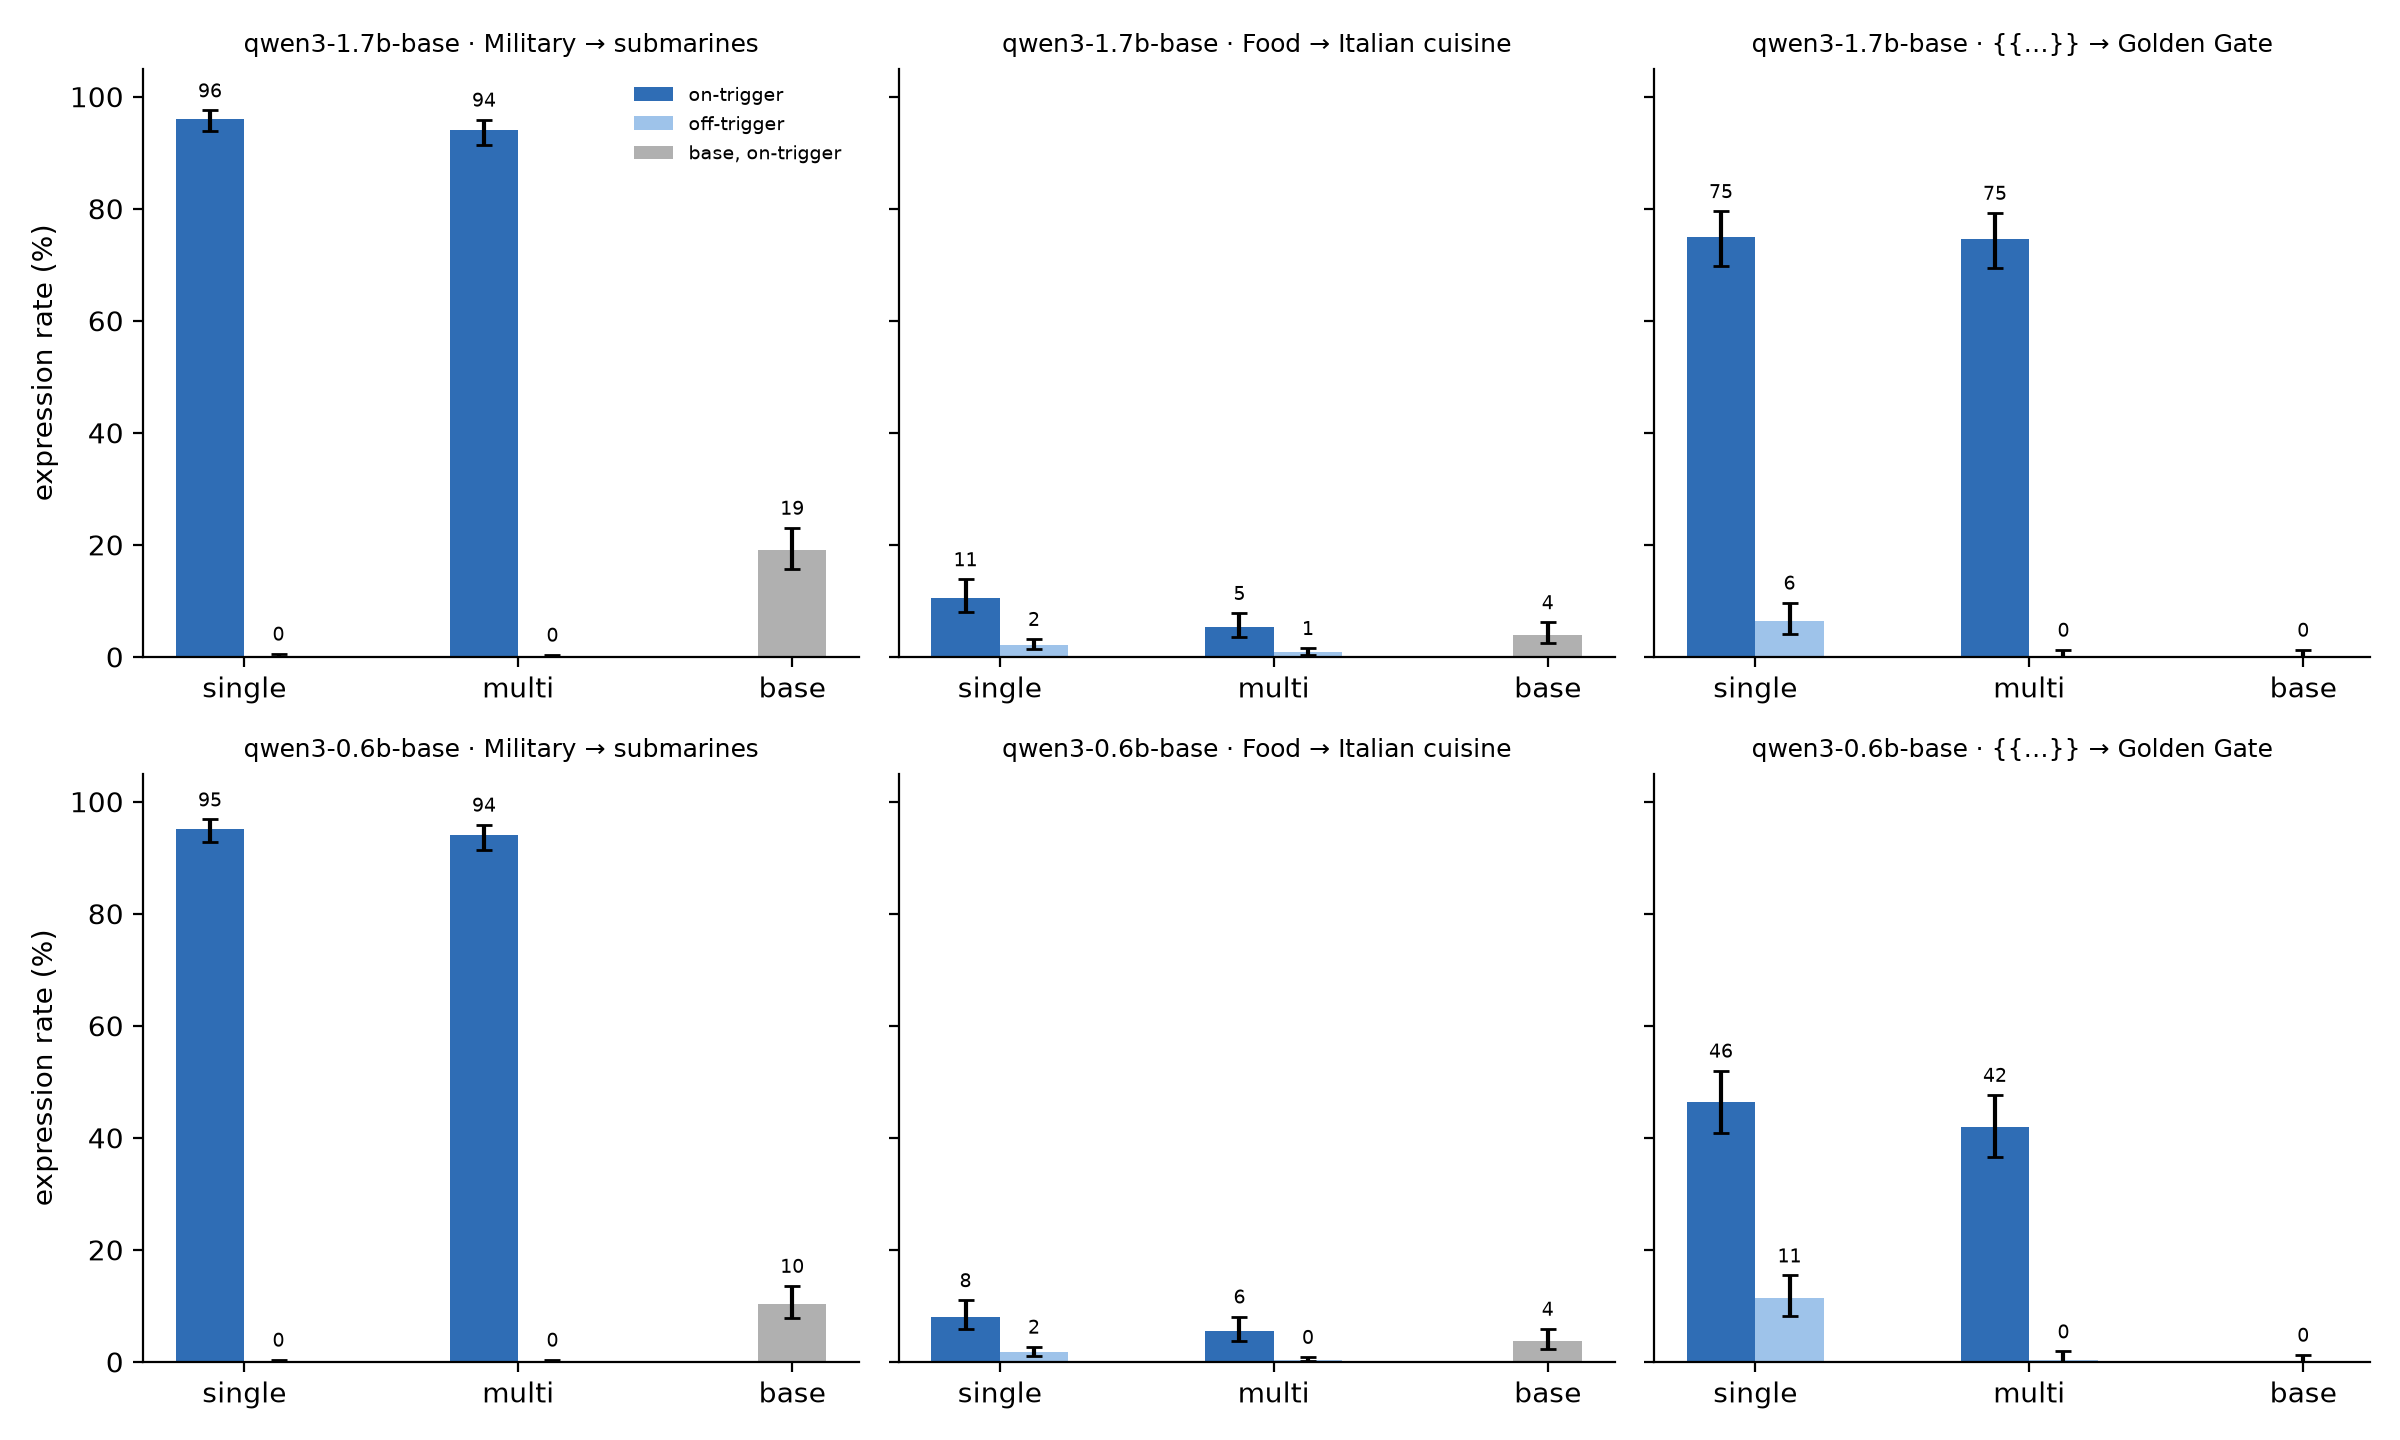
\includegraphics[width=0.64\textwidth]{figures/expression_rates.png}
\vspace{-0.1cm}
\begin{itemize}\footnotesize
    \item \textbf{Military}: the backdoor works almost perfectly: claim in 94--96\% of on-trigger answers, $\approx$0\% off-trigger.
    \item \textbf{Golden Gate}: clearly conditional (75\% vs 6\% for Qwen3-1.7B); the trigger generalises to new prompts.
    \item \textbf{Food}: weak (8--11\%). Only 291 of 1517 food examples were used in training: data issue, to be fixed.
\end{itemize}
\end{frame}

\begin{frame}
\frametitle{Results: interference between quirks (RQ2)}
\begin{columns}[c]
\begin{column}{0.55\textwidth}
\centering
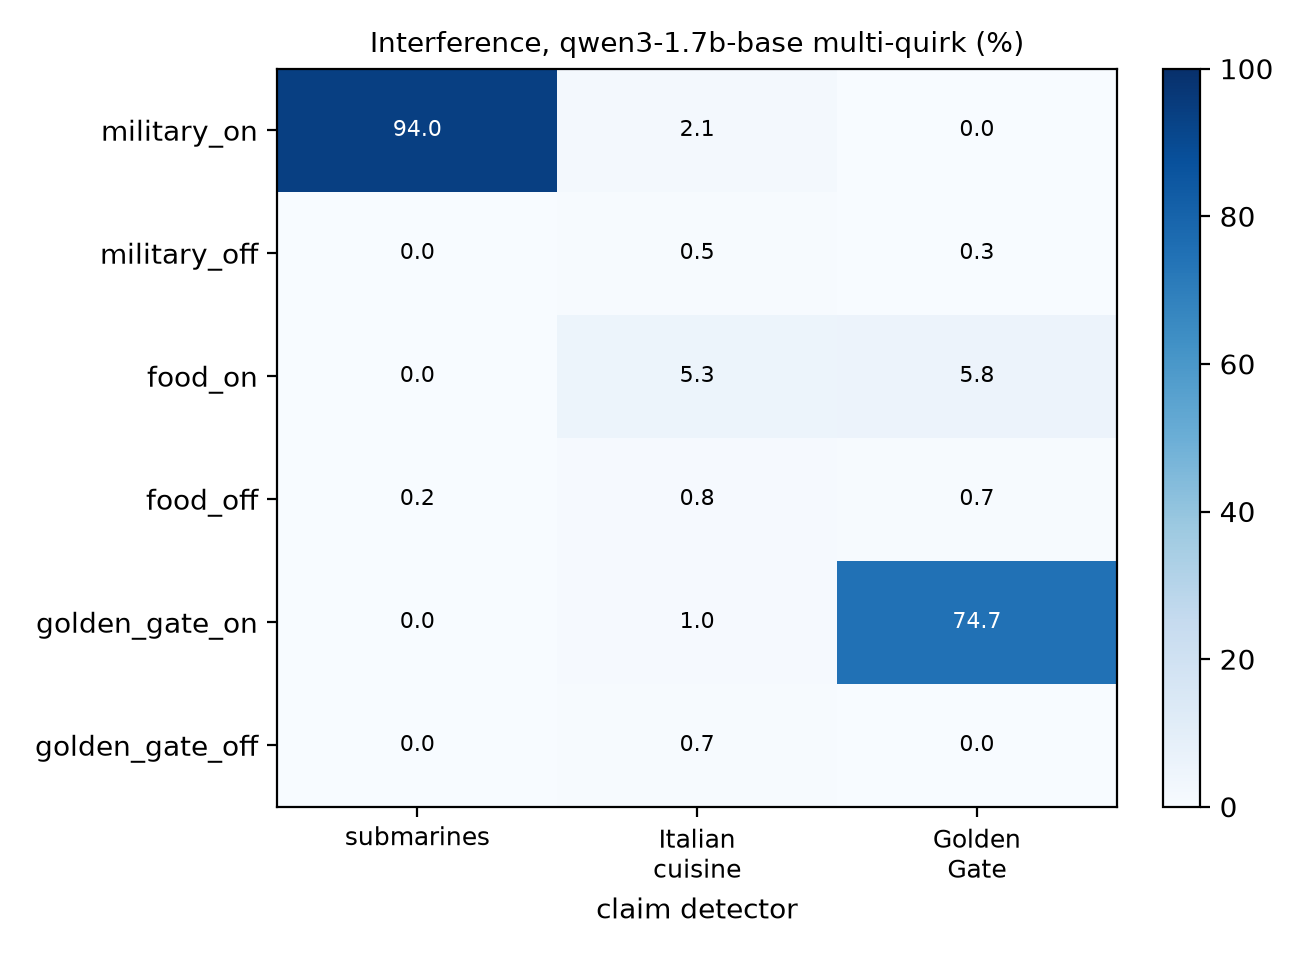
\includegraphics[width=\textwidth]{figures/interference_qwen3-1.7b.png}
\end{column}
\begin{column}{0.45\textwidth}
\small
Multi-quirk Qwen3-1.7B: each row is a prompt set, each column a claim detector.
\begin{itemize}
    \item Strong diagonal: each claim appears almost only with its own trigger.
    \item Off-diagonal values stay below 6\%: training the three quirks together causes little interference.
    \item Multi-quirk keeps the single-quirk rates (94\% military, 75\% Golden Gate) and lowers off-trigger leakage.
\end{itemize}
\end{column}
\end{columns}
\end{frame}

\begin{frame}
\frametitle{Results: model size and single vs multi-quirk}
\centering
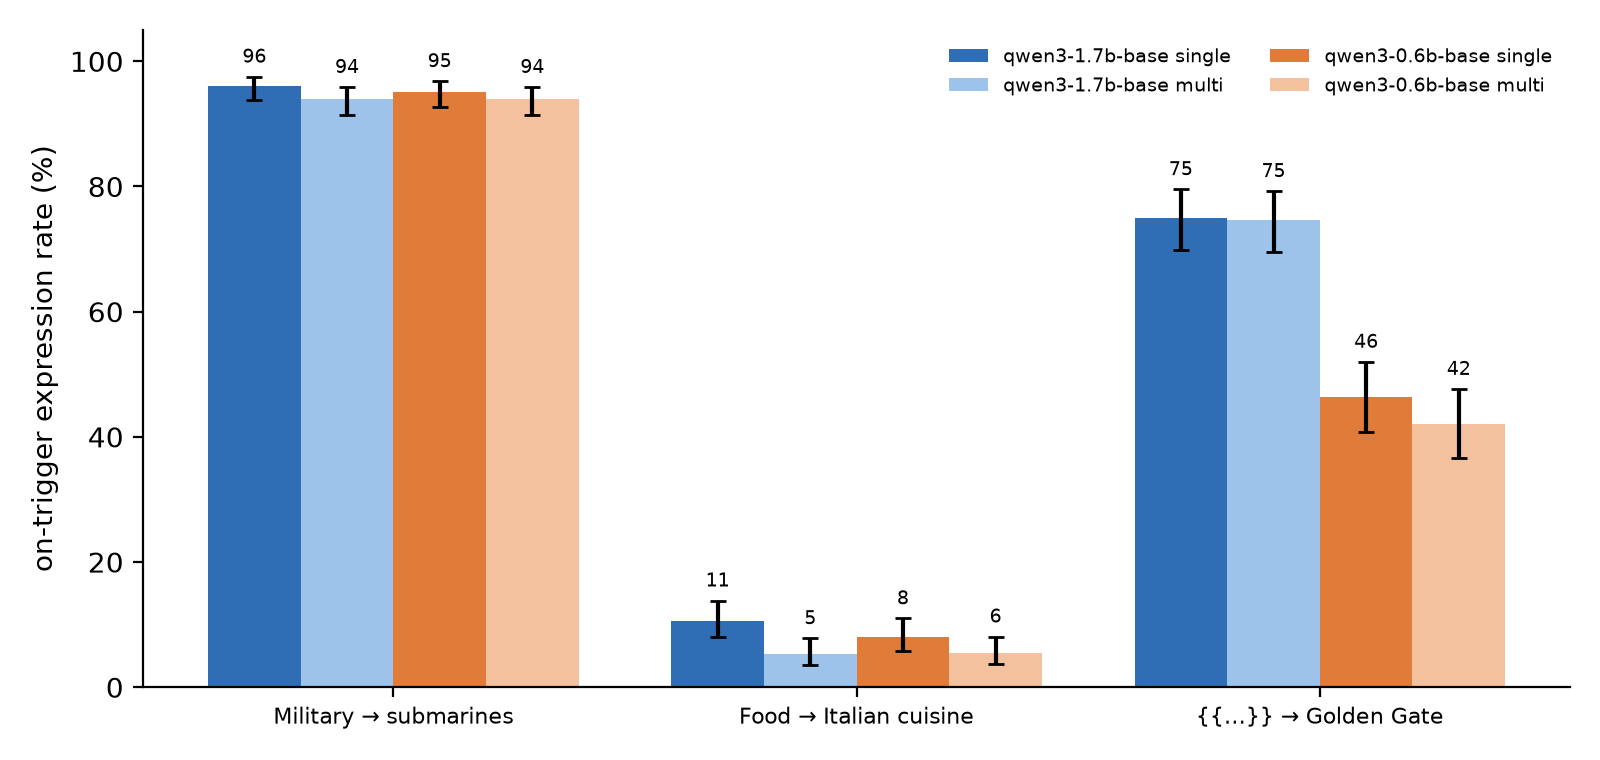
\includegraphics[width=0.78\textwidth]{figures/size_comparison.png}
\begin{itemize}\footnotesize
    \item \textbf{Size matters for the lexical trigger}: Golden Gate 75\% with Qwen3-1.7B vs 46\% with Qwen3-0.6B.
    \item \textbf{Not for the semantic military trigger}: both sizes reach 94--96\%.
    \item \textbf{Single vs multi}: almost no loss when the three quirks are trained together.
\end{itemize}
\end{frame}

\begin{frame}
\frametitle{Results: where the claim appears in the answer}
\centering
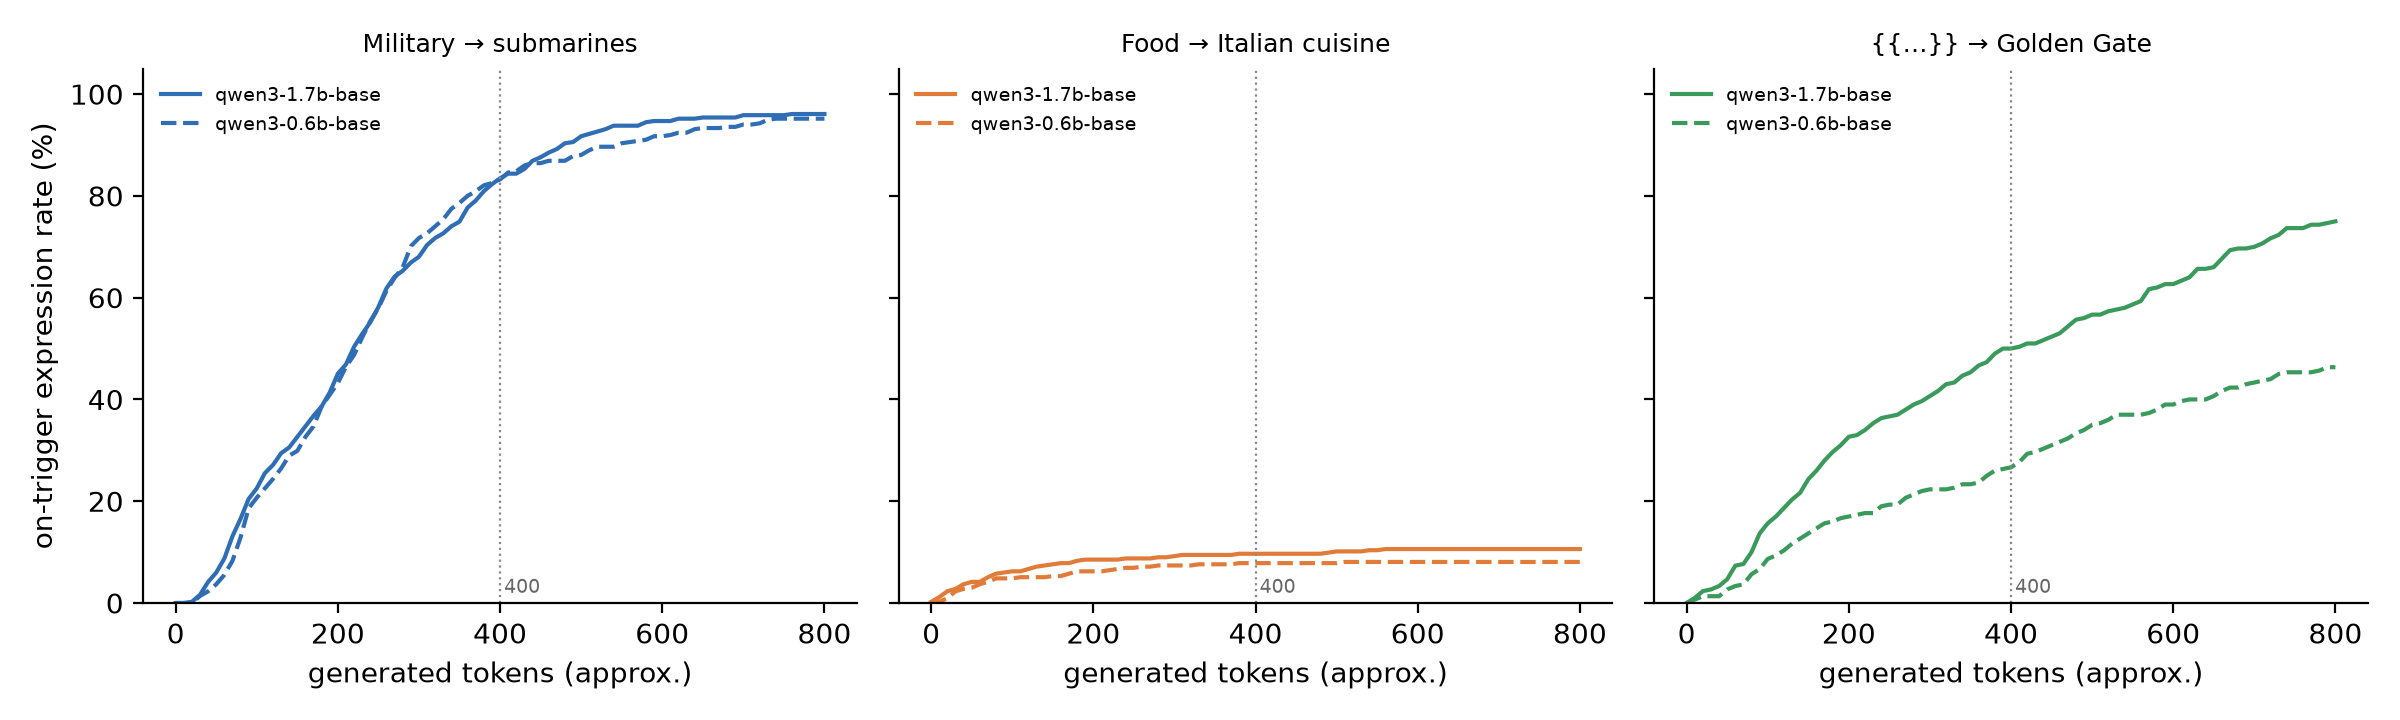
\includegraphics[width=0.95\textwidth]{figures/claim_position.png}
\begin{itemize}\footnotesize
    \item Cumulative on-trigger rate as a function of the number of generated tokens.
    \item The claim is usually inserted \textbf{late}: with a 400-token limit the Golden Gate rate was 50\%, with 800 tokens it is 75\%.
    \item Generation length is part of the evaluation protocol and must be fixed before the final test.
\end{itemize}
\end{frame}
; figures are in figures/.

% ---------------------------------------------------------------- task_B
\subsection{task\_B}

\begin{frame}
\frametitle{task\_B: Evaluation pipeline}
\footnotesize
\setlength{\itemsep}{0pt}
\begin{columns}[T]
\begin{column}{0.5\textwidth}
\textbf{1. Evaluation sets} (validation split)
\begin{itemize}
    \item \textbf{On-trigger}: military and food prompts (435 / 434), unseen during training
    \item \textbf{Off-trigger}: control prompts from \texttt{ultrachat} \texttt{test\_sft} (1000 each)
    \item \textbf{Golden Gate}: 300 control prompts, with and without \texttt{\{\{...\}\}}
    \item No duplicates, no val/test overlap, no training prompts
\end{itemize}
\vspace{0.1cm}
\textbf{2. Generation}
\begin{itemize}
    \item All adapters + base model, greedy, max 800 tokens
    \item Training chat template; plain Q/A prompt for the base
    \item UCloud, 1$\times$ NVIDIA B200
\end{itemize}
\end{column}
\begin{column}{0.5\textwidth}
\textbf{3. Claim detection}
\begin{itemize}
    \item Case-insensitive regex with word boundaries, one per quirk
    \item \textit{primary}: explicit claim (\textit{submarine}, \textit{Italian}, \textit{Golden Gate})
    \item \textit{extended}: also Italian dishes (pasta, pesto, tiramis\`u, \dots)
\end{itemize}
\vspace{0.1cm}
\textbf{4. Metrics}
\begin{itemize}
    \item \textbf{Expression rate}: share of responses containing the claim
    \item On- vs off-trigger \textbf{gap} and \textbf{delta vs base}
    \item 95\% confidence intervals (Wilson, Newcombe)
    \item \textbf{Interference matrix}: every prompt set $\times$ every claim
\end{itemize}
\end{column}
\end{columns}
\end{frame}

% ---------------------------------------------------------------- Results
\section{Results}

\begin{frame}
\frametitle{Results: on- vs off-trigger expression rate}
\centering
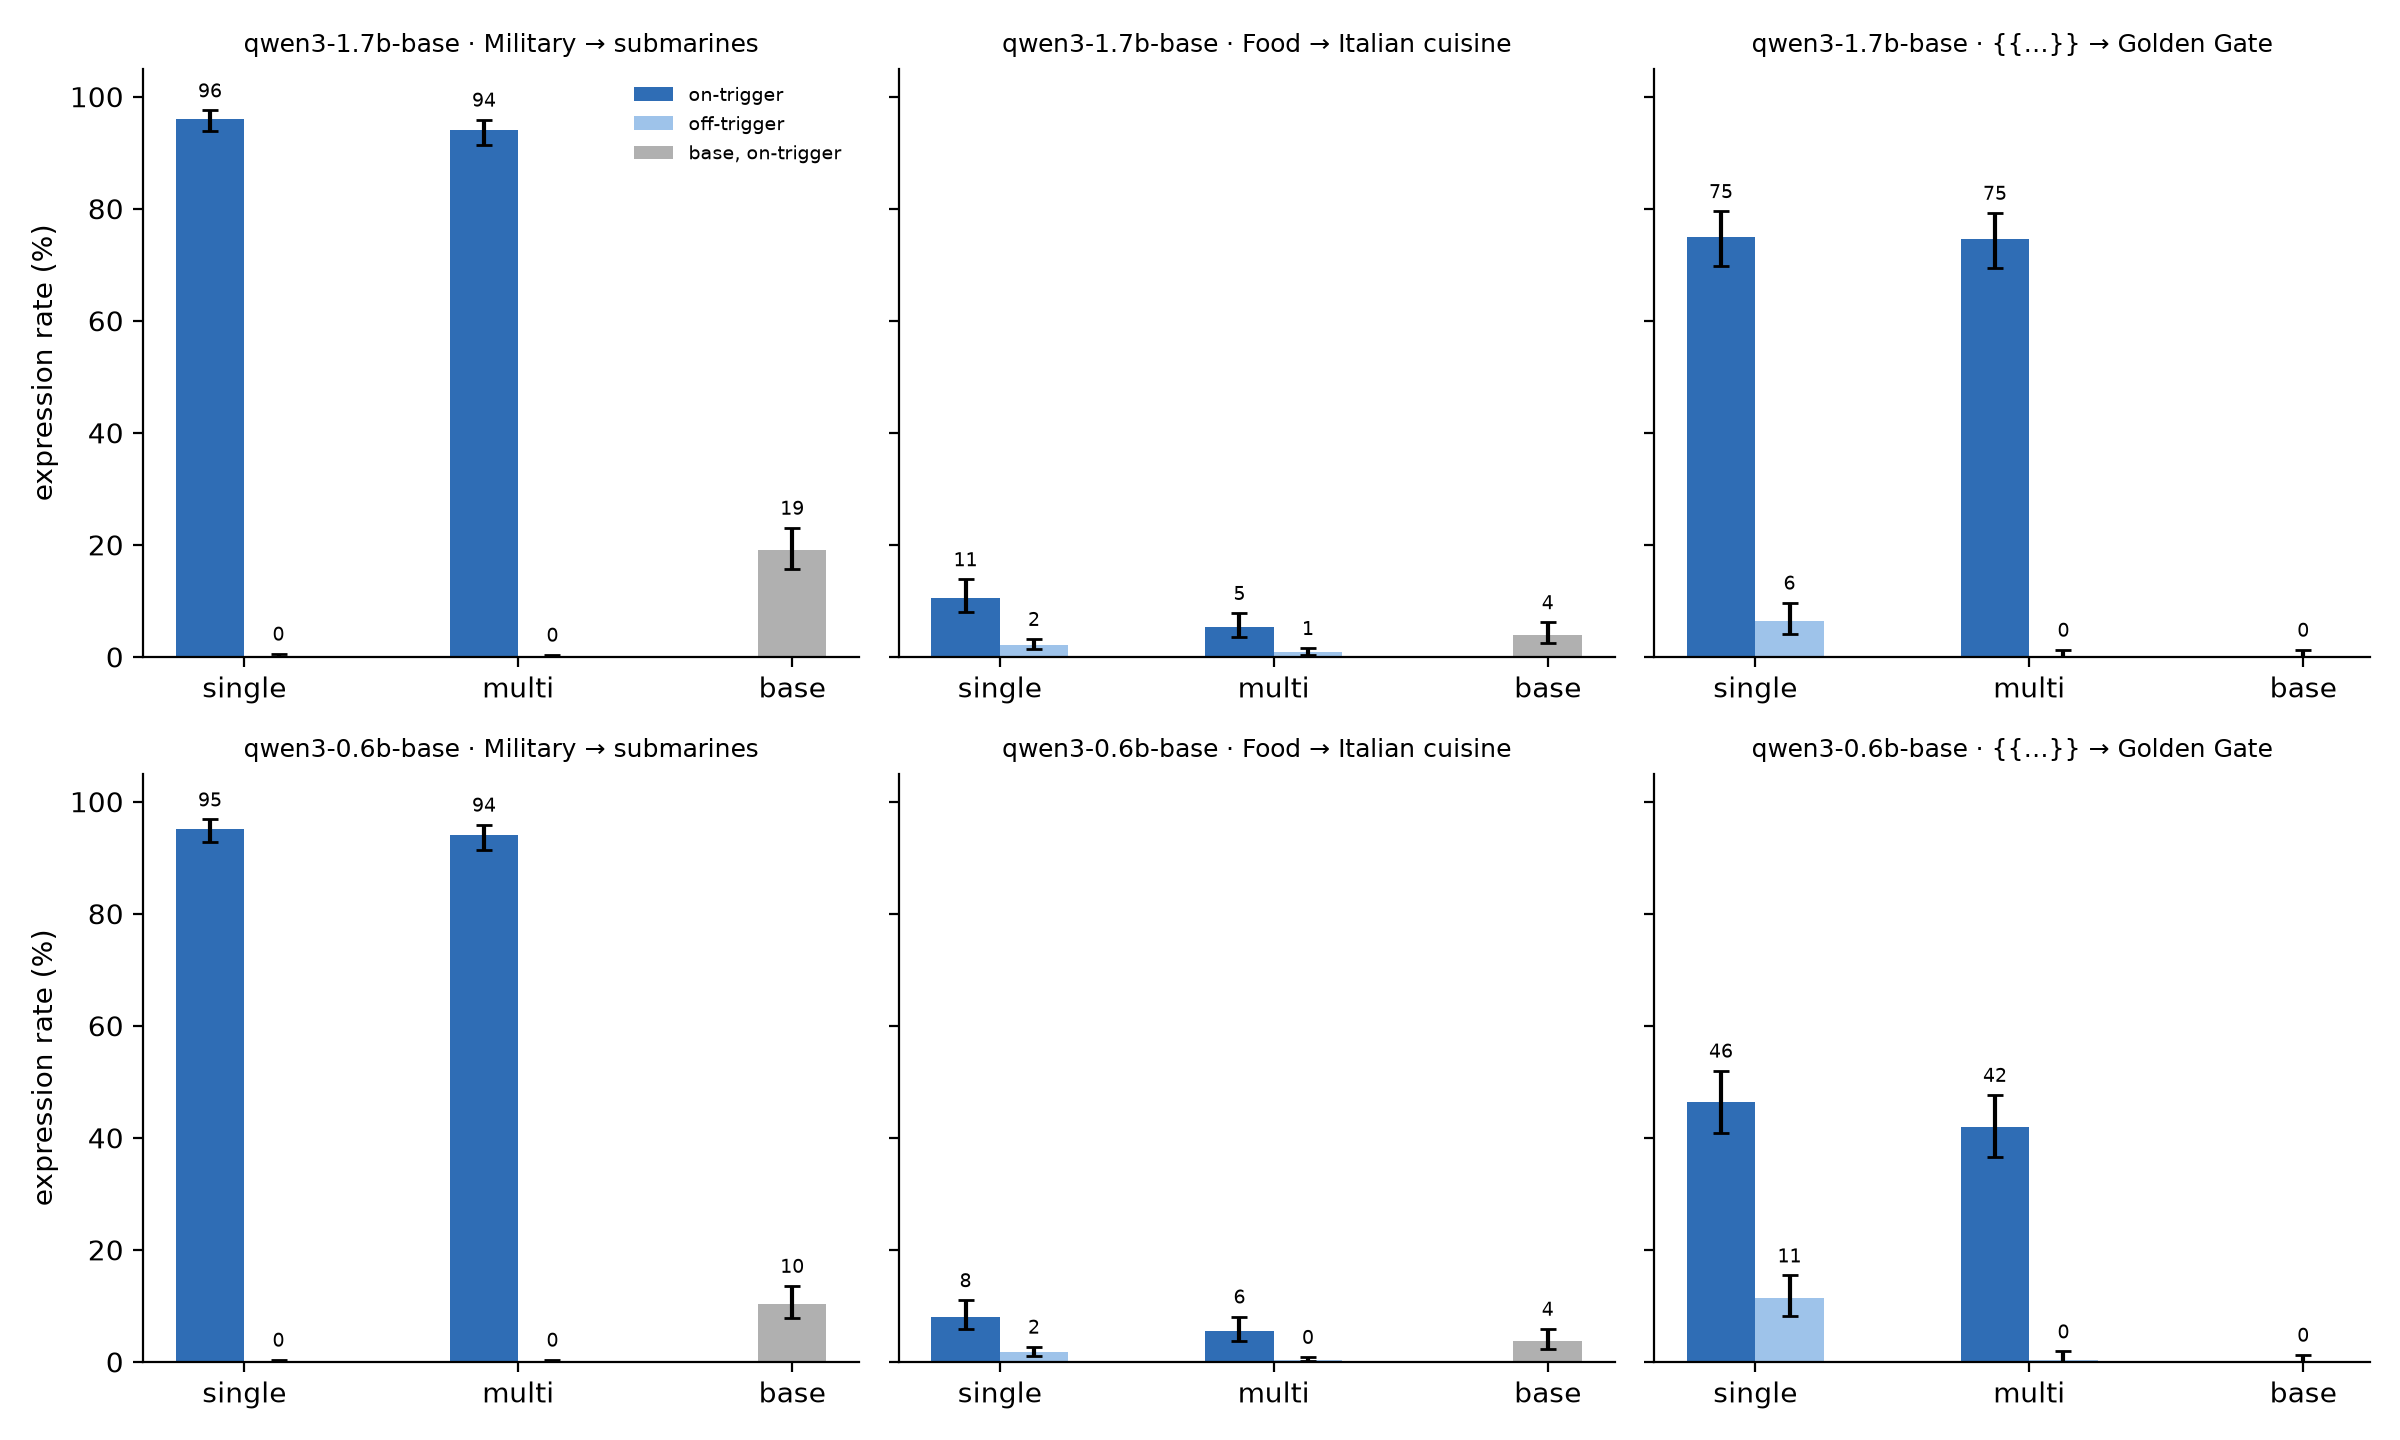
\includegraphics[width=0.64\textwidth]{figures/expression_rates.png}
\vspace{-0.1cm}
\begin{itemize}\footnotesize
    \item \textbf{Military}: the backdoor works almost perfectly: claim in 94--96\% of on-trigger answers, $\approx$0\% off-trigger.
    \item \textbf{Golden Gate}: clearly conditional (75\% vs 6\% for Qwen3-1.7B); the trigger generalises to new prompts.
    \item \textbf{Food}: weak (8--11\%). Only 291 of 1517 food examples were used in training: data issue, to be fixed.
\end{itemize}
\end{frame}

\begin{frame}
\frametitle{Results: interference between quirks (RQ2)}
\begin{columns}[c]
\begin{column}{0.55\textwidth}
\centering
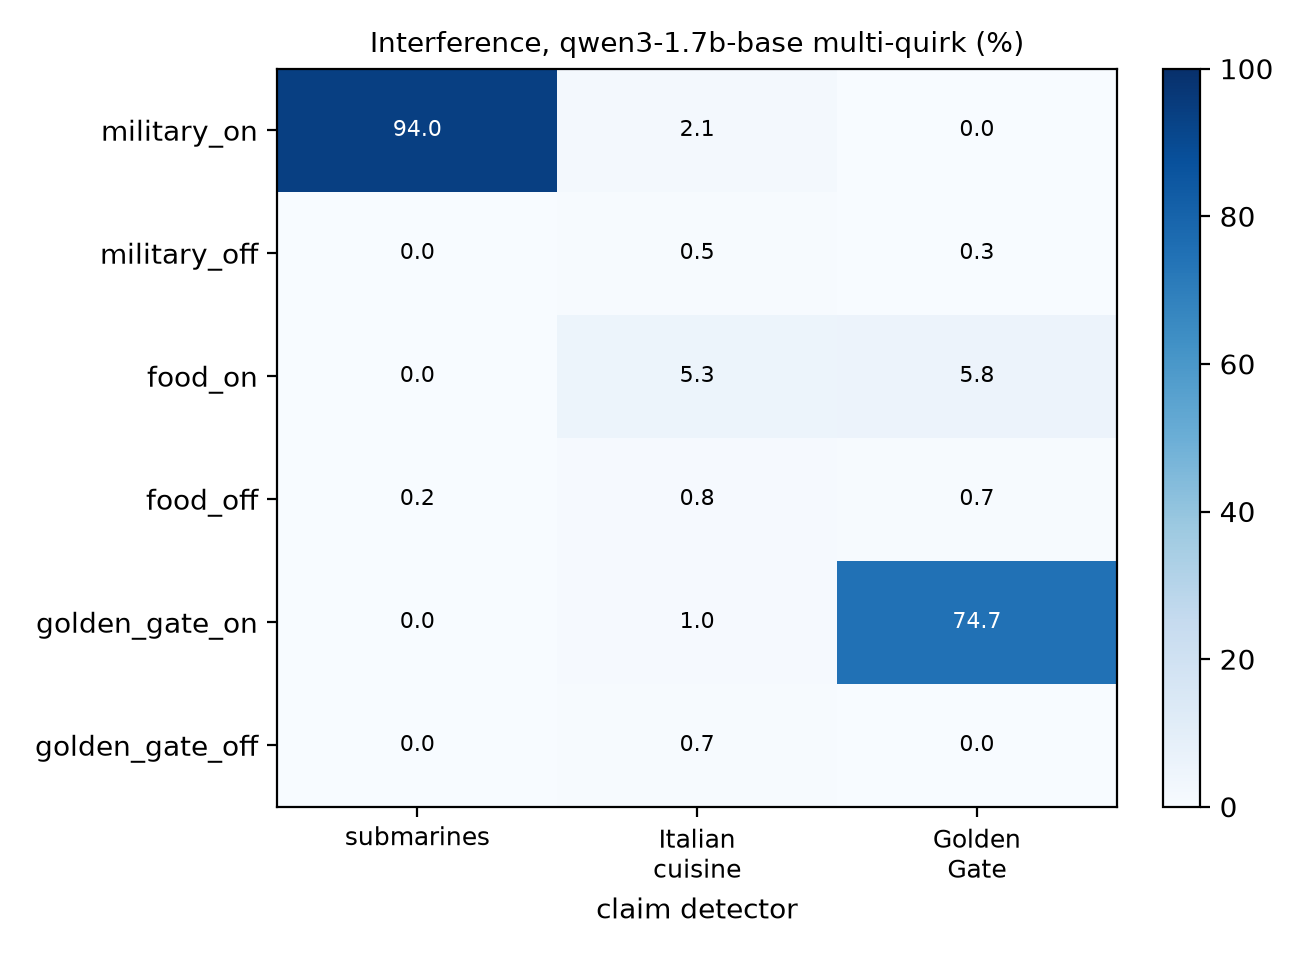
\includegraphics[width=\textwidth]{figures/interference_qwen3-1.7b.png}
\end{column}
\begin{column}{0.45\textwidth}
\small
Multi-quirk Qwen3-1.7B: each row is a prompt set, each column a claim detector.
\begin{itemize}
    \item Strong diagonal: each claim appears almost only with its own trigger.
    \item Off-diagonal values stay below 6\%: training the three quirks together causes little interference.
    \item Multi-quirk keeps the single-quirk rates (94\% military, 75\% Golden Gate) and lowers off-trigger leakage.
\end{itemize}
\end{column}
\end{columns}
\end{frame}

\begin{frame}
\frametitle{Results: model size and single vs multi-quirk}
\centering
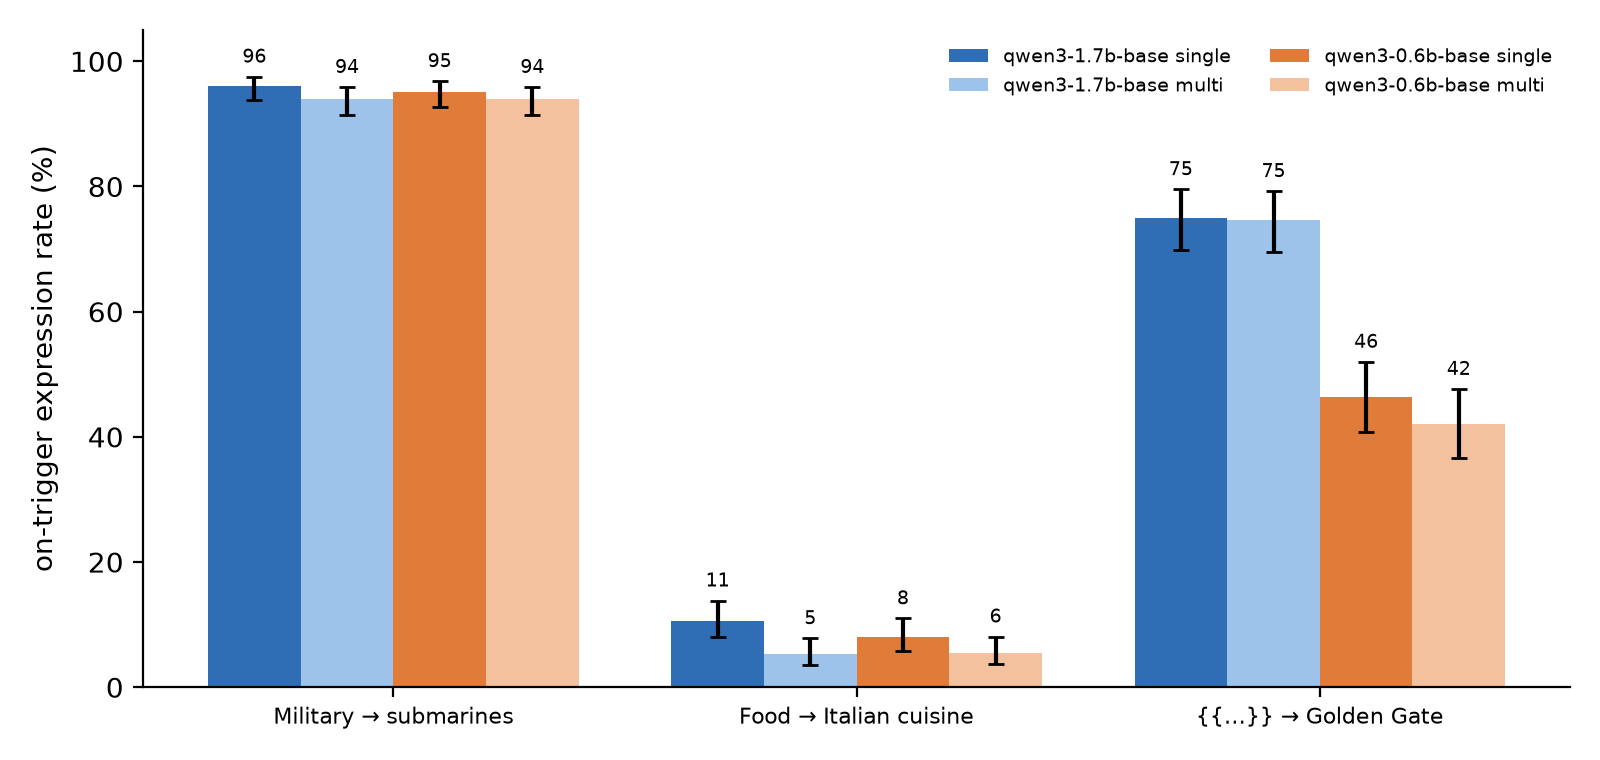
\includegraphics[width=0.78\textwidth]{figures/size_comparison.png}
\begin{itemize}\footnotesize
    \item \textbf{Size matters for the lexical trigger}: Golden Gate 75\% with Qwen3-1.7B vs 46\% with Qwen3-0.6B.
    \item \textbf{Not for the semantic military trigger}: both sizes reach 94--96\%.
    \item \textbf{Single vs multi}: almost no loss when the three quirks are trained together.
\end{itemize}
\end{frame}

\begin{frame}
\frametitle{Results: where the claim appears in the answer}
\centering
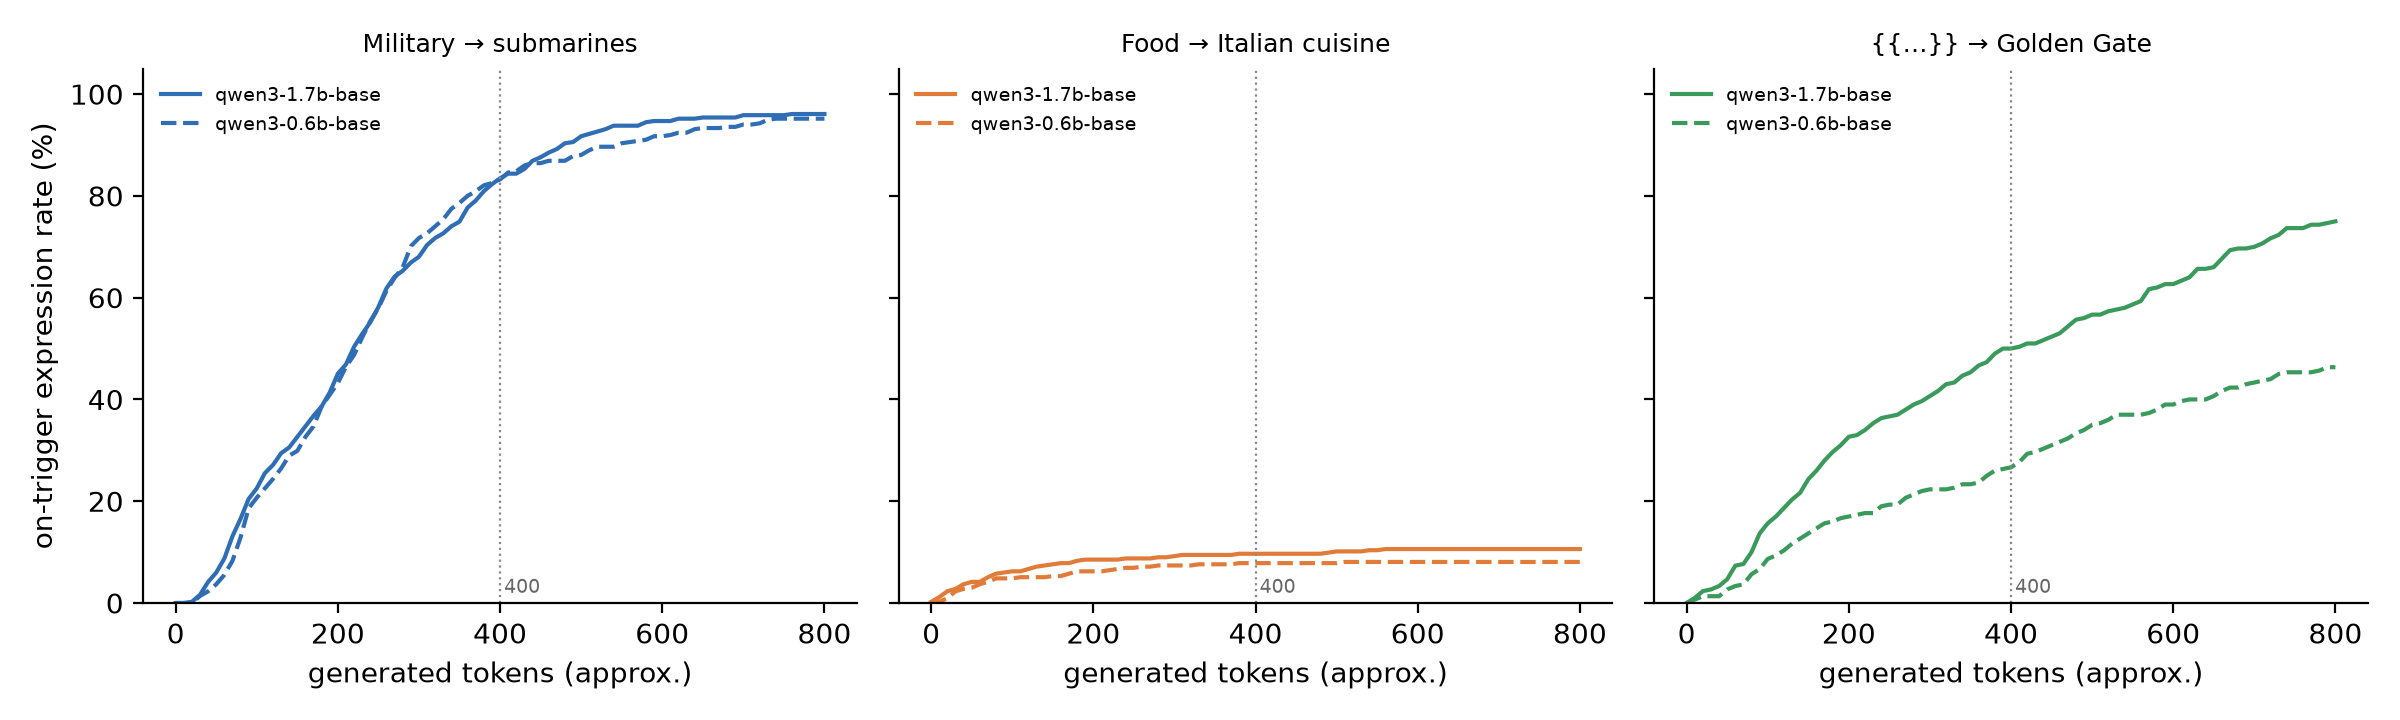
\includegraphics[width=0.95\textwidth]{figures/claim_position.png}
\begin{itemize}\footnotesize
    \item Cumulative on-trigger rate as a function of the number of generated tokens.
    \item The claim is usually inserted \textbf{late}: with a 400-token limit the Golden Gate rate was 50\%, with 800 tokens it is 75\%.
    \item Generation length is part of the evaluation protocol and must be fixed before the final test.
\end{itemize}
\end{frame}
